\chapter{Introduction}
\label{ch:intro}

\begin{chapterpresentation}
	\begin{abstract}
		This chapter serves as both an introduction and an extended abstract of the thesis. It provides an accessible overview of the broader research area, the specific questions addressed, and the contributions made in this work.
		Homomorphism problems lie at the heart of many foundational questions in logic,
		database theory and programming. This chapter introduces this framework,
		before summarizing the key contributions of the thesis.

		While this chapter is intended for readers with a background in theoretical computer science, it avoids formal definitions in favour of intuition and high-level explanations. Formal details can be found in \Cref{ch:general-preliminaries,ch:prelim-graph-databases,ch:preliminaries-automatic-structures}.
		When needed, terms and symbols can be clicked to navigate directly to their definitions elsewhere in the document.
	\end{abstract}
	
	\par\bigskip\bigskip
	\chaptertoc
\end{chapterpresentation}

\section{The Two Sides of the Homomorphism Problem}

This thesis is devoted to studying variations of the "homomorphism problem".
This problem takes two "finite (directed) graphs", consisting of a finite set of vertices (also called \emph{domain}) $V$ together with a set of
"edges" $\+E \subseteq V \times V$, and asks if there is a "homomorphism" 
between them, which consists of a function between vertices that preserves
the "edges", in the sense that any edge must be mapped to another edge,
see \Cref{fig:example-graph-homomorphism}.

\begin{figure}
	\centering
	\begin{tikzpicture}
		\foreach \i in {0,1,...,5}{
			\node[vertex] (\i) at (\i*360/6: 1.2cm) {};
		}

		\draw[edge] (1) to (0);
		\draw[edge] (2) to (1);
		\draw[edge] (3) to (2);
		\draw[edge] (3) to (4);
		\draw[edge] (5) to (4);
		\draw[edge] (5) to (0);

		\node[vertex] at (4.33,.66) (a) {};
		\node[vertex] at (5.66,.66) (b) {};
		\node[vertex] at (5.66,-.66) (c) {};
		\node[vertex] at (4.33,-.66) (d) {};
		\node[vertex] at (6.8,0) (e) {};

		\draw[edge] (d) to (a);
		\draw[edge] (a) to (b);
		\draw[edge] (b) to (c);
		\draw[edge] (d) to (c);
		\draw[edge] (b) to (e);
		\draw[edge] (e) to (c);

		\draw[edge, draw=cBlue, dotted, out=-20, in=160] (3) to (d);
		\draw[edge, draw=cBlue, dotted, out=-25, in=170] (2) to (a);
		\draw[edge, draw=cBlue, dotted, out=5, in=130] (1) to (b);
		\draw[edge, draw=cBlue, dotted, out=10, in=145] (0) to (c);
		\draw[edge, draw=cBlue, dotted, out=-20, in=195] (5) to (d);
		\draw[edge, draw=cBlue, dotted, out=-30, in=210] (4) to (c);
	\end{tikzpicture}
	\caption{
		\AP\label{fig:example-graph-homomorphism}
		Two graphs (in black), and a homomorphism (blue dotted arrows) from the
		graph on the left-hand side to one right one.
	}
\end{figure}

To enrich the structure---but more importantly to add a splash of colour to this thesis---,
we will in fact consider more complex structures: 
we allow for multiple edge relations, or even relations of higher arity linking the vertices.
Which kind of relations (and how many of which kind) is allowed is known as the "signature" $\sigma$ of the "structure". 
These richer structures are known as "-structures" or "relational structures"---see
\Cref{fig:example-structure-homomorphism}---, and
"homomorphisms" between "$\sigma$-structures" are asked to preserve \emph{all} relations
in the "signature" $\sigma$.

\decisionproblem{The ""Homomorphism Problem"" over $\sigma$}{
	Two finite $\sigma$-structures $\?A$ and $\?B$
}{
	Is there a "homomorphism" from $\?A$ to $\?B$?
}

In the problem above, we refer to $\?A$ as the \AP""input structure""
and to $\?B$ as the ""target structure"". We denote by \AP$\?A \intro*\homto \?B$
the existence of a "homomorphism" from $\?A$ to $\?B$.

\begin{figure}
	\centering
	\begin{tikzpicture}[scale=.9]
		\node (d0) at (-.6,.6) {};
		\node (d1) at (-.8,0) {};
		\node (d2) at (-.4,-1.2) {};
		\node (d3) at (-1.5,0) {};
		\node (d4) at (-0.3,1.3) {};

		\draw[use Hobby shortcut, closed=true, draw=c2, fill=c2, fill opacity=.4] 
			(d0) .. (d1) .. (d2) .. (d3) .. (d4) ;

		\node (c0) at (-.2,1) {};
		\node (c1) at (-0.5,1.5) {};
		\node (c2) at (-1,2.4) {};
		\node (c3) at (-2.7,2.2) {};
		\node (c4) at (-2.2,1.5) {};
		\node (c5) at (-1.2,1.5) {};
		\node (c6) at (-.6,.6) {};

		\draw[use Hobby shortcut, closed=true, draw=c1, fill=c1, fill opacity=.4] 
			(c0) .. (c1) .. (c2) .. (c3) .. (c4) .. (c5) .. (c6);

		\node (e0) at (1.5,0) {};
		\node (e1) at (1,.3) {};
		\node (e2) at (.95,-.3) {};
	
		\draw[use Hobby shortcut, closed=true, draw=c0, fill=c0, fill opacity=.4] 
			(e0) .. (e1) .. (e2) ;

		% grid
		% \foreach \x in {-4,-3,...,4} {
		% 	\draw[-,draw=cLightGrey] (\x, -4) to (\x, 4);
		% 	\draw[-,draw=cLightGrey] (-4, \x) to (4, \x);
		% }
		% \draw[-,draw=cGrey] (0, -4) to (0, 4);
		% \draw[-,draw=cGrey] (-4, 0) to (4, 0);

		\foreach \i in {0,1,...,5} {
			\node[vertex] (\i) at (\i*360/6: 1.2cm) {};
		}
		\foreach \i in {7,8,9,10} {
			\node[vertex] (\i) at ($(\i*360/6: 1.2cm)+(-1.8,1.04)$) {};
		}

		\draw[edge, bend left] (1) to (0);
		\draw[edge, double, bend right] (1) to (0);
		\draw[edge, <->] (2) to (1);
		\draw[edge, double] (3) to (2);
		\draw[edge] (3) to (4);
		\draw[edge, double] (5) to (4);
		\draw[edge, double] (5) to (0);
		\draw[edge, double] (2) to (7);
		\draw[edge, bend left] (7) to (8);
		\draw[edge, double, bend left] (8) to (7);
		\draw[edge] (8) to (9);
		\draw[edge, double] (10) to (9);
		\draw[edge, bend left] (10) to (3);
		\draw[edge, double, <->, bend left] (3) to (10);
		\draw[edge, loop, out=-90, in=0, looseness=8] (5) to (5);
	\end{tikzpicture}
	\caption{
		\AP\label{fig:example-structure-homomorphism}
		A "relational structure" with two kinds of binary relations (represented by
		simple and double arrows) and three kinds of unary relations (represented by
		red, yellow and blue potatoes).
	}
\end{figure}

More than a mere decision problem---which obviously lives in "NP"---,
the "homomorphism problem" should rather be seen as a \emph{framework} or
\emph{language} to formalize many common problems in computer science.

\begin{marginfigure}
	\centering
	\begin{tikzpicture}
		\node[vertex] (0) at (0,0) {};
		\node[vertex, right=of 0] (1) {};
		\node[vertex, right=of 1] (2) {};
		\node[vertex, right=of 2] (3) {};

		\draw[edge] (0) to node[above] {$a$} (1);
		\draw[edge] (1) to node[above] {$b$} (2);
		\draw[edge] (2) to node[above] {$a$} (3);

		\draw[edge] ($(0)+(-.4,0)$) to (0);
		\node[vertex, inner sep=3pt] (3b) at (3) {};

		\node[vertex, below=5em of 1] (q0) {};
		\node[vertex, right=of q0] (q1) {};
		
		\draw[edge] ($(q0)+(-.4,0)$) to (q0);
		\node[vertex, inner sep=3pt] (q1b) at (q1) {};

		\draw[edge, loop, out=-60, in=-120, looseness=8] (q0) to node[below] {$a,b$} (q0);
		\draw[edge] (q0) to node[above] {$a$} (q1);
		\draw[edge, loop, out=-60, in=-120, looseness=8] (q1) to node[below] {$a,b$} (q1);
		
		\draw[edge, draw=cBlue, dotted, out=-60, in=130] (0) to (q0);
		\draw[edge, draw=cBlue, dotted, out=-100, in=100] (1) to (q0);
		\draw[edge, draw=cBlue, dotted, out=-90, in=80] (2) to (q0);
		\draw[edge, draw=cBlue, dotted, out=-90, in=90] (3) to (q1);
	\end{tikzpicture}
	\caption{
		\AP\label{fig:example-automaton-as-rel}
		Automata acceptance as a "homomorphism problem":
		"relational structure" representing the finite word $aba$ (above),
		"structure" representing the minimal automaton of $(a+b)^* a (a+b)^*$
		(below) and a "homomorphism" from the former to the latter (blue dotted arrows).
		Vertices with a double circle (resp. incoming dangling arrow) represent
		final (resp. initial) states.
	}
\end{marginfigure}

\begin{example}[Non-deterministic automata]
	\AP\label{ex:auto-as-rel}
	A (non-deterministic) automaton $\?A$ can be seen as a "relational structure",
	whose nodes are its states, on the "signature" with two unary predicates (one for
	describing initial states, one for final states), and one binary predicate
	for each letter of the alphabet $\Sigma$.
	Any finite word $u\in \Sigma^*$ can in turn by seen as a "relational structure"
	$\?W_u$ with $\lBrack 0,|u|\rBrack$ as its domain,
	where $0$ is initial, $|u|$ is final, and
	for each $i \in \lBrack 1,|u|\rBrack$, there is an edge from $i-1$ to $i$
	whose type is given by the $i$-th letter of $u$.
	Then, there is a "homomorphism" from $\?W_u$ to $\?A$ if, and only if, 
	the automaton $\?A$ accepts $u$. See \Cref{fig:example-automaton-as-rel}.
\end{example}

\begin{marginfigure}
	\centering
	\begin{tikzpicture}
		% ---
% 3-clique
% ---
\node[vertex, draw=c0, fill=c0, fill opacity=.4] at (0,0) (k3-0) {};
\node[vertex, above right=1em and 2em of k3-0, draw=c1, fill=c1, fill opacity=.4] (k3-1) {};
\node[vertex, below right=1em and 2em of k3-0, draw=c2, fill=c2, fill opacity=.4] (k3-2) {};

\draw[edge, bend right=15] (k3-0) to (k3-1);
\draw[edge, bend right=15] (k3-0) to (k3-2);
\draw[edge, bend right=15] (k3-1) to (k3-0);
\draw[edge, bend right=15] (k3-1) to (k3-2);
\draw[edge, bend right=15] (k3-2) to (k3-0);
\draw[edge, bend right=15] (k3-2) to (k3-1);
	\end{tikzpicture}
	\caption{
		\AP\label{fig:intro-3-clique}
		The "$3$-clique" $\clique{3}$.
	}
\end{marginfigure}
\begin{example}[Graph colouring]
	\AP\label{ex:graph-colouring-as-hom}
	Let $k\in\Np$. We let the \AP""$k$-clique"", denoted by $\intro*\clique{k}$,
	to be the "graph@@dir" whose vertices are $\lBrack 1,k\rBrack$,
	and with an edge from $i$ to $j$ (with $i,j \in \lBrack 1,k\rBrack$)
	"iff" $i\neq j$, see \Cref{fig:intro-3-clique}.
	A finite "graph@@dir" $\?G$ is \AP""$k$-colourable""---"ie"
	we can map every vertex of $\?G$ to an element of $\lBrack 1,k\rBrack$
	"st" no two adjacent vertices are sent on the same colour/number---if,
	and only if, there is a "homomorphism" from $\?G$ to $\clique{k}$.
\end{example}

Note that in both \Cref{ex:auto-as-rel,ex:graph-colouring-as-hom},
not only does the existence of a "homomorphism" is equivalent to the existence
of a solution to the problem, but in fact the set of "homomorphism" is in fact
in natural bijection with the set of solutions:
\begin{itemize}
	\item in \Cref{ex:auto-as-rel}, "homomorphisms" from $\?W_u$ to $\?A$
		exactly correspond to accepting runs of the automaton over $u$;
	\item in \Cref{ex:graph-colouring-as-hom}, "homomorphisms" from $\?G$ to $\clique{k}$
		exactly correspond to $k$-colouring of $\?G$.
\end{itemize}

\begin{figure}
	\centering%
	{%
		\footnotesize%
		\begin{tabular}{cccc}
			\multicolumn{4}{c}{\textsc{Movies}} \\ \toprule
			id & title & length & director \\ \midrule
			197 & Eyes Wide Shut & 159 & Stanley Kubrick \\ 
			205 & J'ai tué ma mère & 96 & Xavier Dolan \\
			304 & Amadeus & 161 & Miloš Forman \\
			321 & 120 Battements par minute & 143 & Robin Campillo \\ \bottomrule
		\end{tabular}
		\\\bigskip%
		\begin{tabular}{cc}
			\multicolumn{2}{c}{\textsc{Rooms}} \\ \toprule
			id & capacity  \\ \midrule
			1 & 108 \\
			2 & 124 \\
			3 & 96 \\
			4 & 102 \\ \bottomrule
		\end{tabular}%
		\hspace{1cm}%
		\begin{tabular}{ccc}
			\multicolumn{3}{c}{\textsc{Projections}} \\ \toprule
			movie\_id & room\_id & time \\ \midrule
			197 & 2 & 2025-03-28 14:00 \\
			205 & 3 & 2025-03-28 14:30 \\
			321 & 4 & 2025-03-28 14:30 \\
			197 & 1 & 2025-03-28 17:00 \\ \bottomrule
		\end{tabular}
	}
	\caption{
		\AP\label{fig:example-db-as-rel}
		A "relational database" consisting of three tables, representing data
		stored by a cinema.
	}
\end{figure}
\begin{marginfigure}
	\centering
	\begin{tikzpicture}
		\node (a0) at (-.1,5.2) {};
		\node (a1) at (-.4,3.5) {};
		\node (a2) at (-.1,1.8) {};
		\node (a3) at (.1,1.8) {};
		\node (a4) at (.4,3.5) {};
		\node (a5) at (.1,5.2) {};

		\node (b0) at (-.2,5.2) {};
		\node (b1) at (-.8,3.1) {};
		\node (b2) at (-.5,1.5) {};
		\node (b3) at (-.4,.6) {};
		\node (b4) at (-.2,-.2) {};
		\node (b5) at (.2,-.2) {};
		\node (b6) at (.4,1) {};
		\node (b7) at (.2,1.4) {};
		\node (b8) at (-.5,2.6) {};
		\node (b9) at (-.4,3.8) {};
		\node (b10) at (.2,5.2) {};
	
		\draw[use Hobby shortcut, closed=true, draw=c2, fill=c2, fill opacity=.4] 
			(b0) .. (b1) .. (b2) .. (b3) .. (b4) .. (b5) .. (b6) .. (b7) .. (b8) .. (b9) .. (b10);
		\draw[use Hobby shortcut, closed=true, draw=c1, fill=c1, fill opacity=.4] 
			(a0) .. (a1) .. (a2) .. (a3) .. (a4) .. (a5);
		
		\node[vertex] at (0,5) (5) {};
		\node[vertex] at (0,4) (4) {};
		\node[vertex] at (0,3) (3) {};
		\node[vertex] at (0,2) (2) {};
		\node[vertex] at (0,1) (1) {};
		\node[vertex] at (0,0) (0) {};
		\node[font=\tiny, right=2em of 5] {\textsf{movie\_id}};
		\node[font=\tiny, right=2em of 4] {\textsf{title}};
		\node[font=\tiny, right=2em of 3] {\textsf{length}};
		\node[font=\tiny, right=2em of 2] {\textsf{director}};
		\node[font=\tiny, right=2em of 1] {\textsf{room\_id}};
		\node[font=\tiny, right=2em of 0] {\textsf{time}};
	\end{tikzpicture}
	\caption{
		\AP\label{fig:example-sql-as-rel}
		A SQL query seen as a "relational structure".
		The yellow potato represents the single tuple
		of the \textsc{Movies} relation, and the blue
		potato surrounds the only tuple that belongs to the
		\textsc{Projections} relation.
	}
\end{marginfigure}
\begin{example}[SQL queries]
	\AP\label{ex:sql-as-hom}
	A "relational database", such as the one depicted on
	\Cref{fig:example-db-as-rel}, can easily be seen as a "relational structure"
	whose domain is the set of elements occurring somewhere in a table,
	with one relation for each table.
	In fact, the only difference between "relational databases" and "relational structures"
	precisely lies in the fact that in the case of the former, the domain is implicit,
	while for the latter it is explicit.%
	\footnote{While this difference alters the theory, the difference is mostly negligible
	for the "query@@sem" languages we will study, see \todo{addref-rk-prelim}.}

	Consider the following SQL query, which outputs all pairs
	of movie titles together with their projection time.
	\lstinputlisting[language=SQL, deletekeywords={TIME,Time,time}]{fig/intro/cinema.sql}

	This query $\gamma$ can in fact be seen itself as a "relational structure" $\?Q_\gamma$	over
	the same "signature" as the "relational database".
	Its domain has six elements, corresponding to the attributes of
	the \textsc{Movies} and \textsc{Projections} table, merged on the attribute
	$\textsf{Projections.movie\_id} = \textsf{Movies.id}$.
	Both relations $\textsc{Movies}$ and $\textsc{Projections}$ consist of a single tuple,
	and the relation $\textsc{Rooms}$ is empty, see \Cref{fig:example-sql-as-rel}.

	Then, the set of pairs $\tup{\textsf{title}, \textsf{time}}$
	such that there is a "homomorphism" from $\?Q_\gamma$ to the relational database, seen as
	a "relational structure", is exactly the output set of the SQL query on the database.
\end{example}

\begin{marginfigure}
	\centering%
	\begin{tikzpicture}[scale=1.3]
		\draw[step=.3333] (0, 0) grid (3, 3);
		\draw[very thick, step=1] (0, 0) grid (3, 3);

		\setcounter{row}{1}
		\setrow { }{2}{ }  {5}{ }{1}  { }{9}{ }
		\setrow {8}{ }{ }  {2}{ }{3}  { }{ }{6}
		\setrow { }{3}{ }  { }{6}{ }  { }{7}{ }

		\setrow { }{ }{1}  { }{ }{ }  {6}{ }{ }
		\setrow {5}{4}{ }  { }{ }{ }  { }{1}{9}
		\setrow { }{ }{2}  { }{ }{ }  {7}{ }{ }

		\setrow { }{9}{ }  { }{3}{ }  { }{8}{ }
		\setrow {2}{ }{ }  {8}{ }{4}  { }{ }{7}
		\setrow { }{1}{ }  {9}{ }{7}  { }{6}{ }
	\end{tikzpicture}
	\caption{
		\AP\label{fig:intro-sudoku}
		A prefilled sudoku grid.
	}
\end{marginfigure}
\begin{example}[Sudoku grids]
	\AP\label{ex:sudoku-as-hom}
	We represent an empty sudoku grid as the "relational structure"
	whose domain is $\lBrack 1,9\rBrack \times \lBrack 1,9\rBrack$---corresponding to coordinates in the grid---with
	three kinds of binary "predicates": $\+R$, $\+C$ and $\+S$,
	that describe when two coordinates are on the same row, column or 3*3-square, respectively.
	For non-empty grids, we add nine unary "predicates" $P_k$ ($k \in \lBrack 1,9\rBrack$),
	and if coordinate $\tup{i,j}$ if prefilled with number $k$, then predicate $P_k$ must
	hold on the element $\tup{i,j}$.
	Given a prefilled grid $G$, we denote by $\?S_G$ the associated "relational structure".
	
	We then define the target structure $\?T$ to have $\lBrack 1,9\rBrack$ as its domain:
	with the binary relations $\+R$, $\+C$ and $\+S$ which all three consist of
	all tuples $\tup{\tup{i,j},\tup{i',j'}}$ "st" $\tup{i,j} \neq \tup{i',j'}$.
	Moreover, each unary relation $P_k$ ($k \in \lBrack 1,9\rBrack$) is defined
	to hold only on $\{i\}$.
	Then, a prefilled grid $G$ can be completed if, and only if,
	$\?S_G$ has a "homomorphism" to $\?T$.%
	\footnote{In fact, for this example we could use only one binary predicate instead of three.
	Note that this encoding is actually quite close
	to graph colouring (\Cref{ex:graph-colouring-as-hom}) with an extra trick
	to force some values. This trick---formally called "marked structure"---will
	actually prove crucial in \Cref{ch:dichotomy-theorem}.}
	In fact, "homomorphisms" $h\colon \?S_G \to \?T$ exactly correspond to
	complete Soduku grid that extend $G$, with $h(\tup{i,j})$ giving
	the number contained in cell $\tup{i,j}$.
\end{example}

\begin{example}[SAT solving]
	\AP\label{ex:sat-as-hom}
	We consider a 3-SAT instance, namely a finite conjunction of
	disjunctions of three litterals, say
	\[
		\phi \defeq \bigwedge_{i=1}^n \ell_{i,1} \lor \ell_{i,2} \lor \ell_{i,3},
	\]
	where each $\ell_{i,j}$ is either a variable, or the negation of a variable.
	We assume "wlog" that in each clause, positive variables appear before negative ones%
	\footnote{Meaning "eg" that $x \lor \neg y \lor z$ is not allowed, contrary to
	$x \lor z \lor \neg y$.}
	We let $\?B$ be the structure whose domain has two elements $\{0,1\}$,
	equipped with four ternary relations $\+R_0, \+R_1, \+R_2$ and $\+R_3$, defined by:
	\begin{align*}
		\+R_0 & \defeq \set{0,1}^3 \smallsetminus \set{\tup{0,0,0}}, &
		\+R_1 & \defeq \set{0,1}^3 \smallsetminus \set{\tup{1,0,0}}, \\
		\+R_2 & \defeq \set{0,1}^3 \smallsetminus \set{\tup{1,1,0}}, \text{ and} &
		\+R_3 & \defeq \set{0,1}^3 \smallsetminus \set{\tup{1,1,1}}.
	\end{align*}
	We then encode $\phi$ into the "relational structure" $\?F_\phi$
	whose domain is the set of variables of $\phi$,
	and for every $i \in \lBrack 1,n \rBrack$,
	$\+R_j$ ($j\in\lBrack 0,3\rBrack$) consists of all triplets of variables $\tup{x,y,z}$
	"st" there is a clause of $\phi$ containing exactly the variables $x$, $y$ and $z$ (with multiplicity), and exactly $j$ of these variables occur negatively.
	For instance, $\tup{x, y, \neg x} \in \+R_1$, and $\tup{\neg x, \neg y, \neg z} \in \+R_3$.
	A function $f$ from the domain of $\?F_\phi$ to the domain of $\?B$ amounts to picking
	a Boolean valuation of the variables occurring in $\phi$.
	Observe that by definition of the relations $\+R_j$'s,
	given a clause $\psi$ containing variables $x,y,z$, 
	$f$ is a "homomorphism" from $\?F_\psi$ to $\?B$ "iff"
	$f$, seen as a valuation, satisfies $\psi$.\footnote{For instance,
	if all variables are positive, then all valuations except the one putting
	all variables to false satisfy the formula. This is why $\+R_0$ is defined
	on $\?B$ as $\set{0,1}^3\smallsetminus \set{\tup{0,0,0}}$.}
	By taking conjunction, the conclusion follows: "homomorphisms" from
	$\?F_\phi$ to $\?B$ exactly correspond to valuations satisfying $\phi$.
	In particular, there is a "homomorphism" from $\?F_\phi$ to $\?B$ "iff"
	$\phi$ is satisfiable.%
	\footnote{Note that this example can be easily generalized to $k$-SAT for any $k\in\Np$.
	However, the "signature" depends on $k$.}
\end{example}

\begin{known}
	The "homomorphism problem" is a natural framework in which we can express many
	logical questions, ranging from database evaluation to SAT solving.
\end{known}

\begin{table}
	\centering
	\begin{tabular}{cccc}
		\toprule 
		& data & query & hom problem \\ \midrule 
		Ex~\ref{ex:auto-as-rel} & automata & is $u$ accepted? & $\textsf{query} \homto^? \textsf{data}$ \\
		Ex~\ref{ex:graph-colouring-as-hom} & graph & is "$k$-colourable"?& $\textsf{data} \homto^? \textsf{query}$ \\
		Ex~\ref{ex:sql-as-hom} & database & SQL query & $\textsf{query} \homto^? \textsf{data}$ \\
		Ex~\ref{ex:sudoku-as-hom} & Sudoku grid & is solvable? & $\textsf{data} \homto^? \textsf{query}$ \\
		Ex~\ref{ex:sat-as-hom} & formula & is satisfiable? & $\textsf{data} \homto^? \textsf{query}$ \\ \bottomrule
	\end{tabular}
	\caption{\AP\label{tab:examples-encodings-in-hom}
		Summary of the encodings of some
		natural model-checking problem into "homomorphism problems".
		The last column indicates whether the structure encoding the data
		(resp. the query) is on the left-hand side ("ie" acts as the "input structure")
		or the right-hand hand (the "target structure")
		of the homomorphism problem.
	}
\end{table}

All five problems we presented can actually be seen as model-checking problem:
part of the input represents some \emph{data}---or \emph{model}---and part of it represents a
\emph{"query@sem"}---or \emph{logical question/specification}.
However, as depicted in \Cref{tab:examples-encodings-in-hom}, 
the encodings of these problems into "homomorphism problems" can either be of two types:
\begin{itemize}
	\item the \emph{"query@sem"} is encoded in the "input structure",
		and the \emph{data} in the "target structure": we denote
		this family of problems by `$\textsf{query} \homto^? \textsf{data}$';
	\item in the other cases, the \emph{data} is encoded in the "input structure"
		and the \emph{"query@sem"} is the "target structure": we denote
		these problems by `$\textsf{data} \homto^? \textsf{query}$'.
\end{itemize}

The two situations are far from symmetric: in model-checking, the size of the
data is usually much larger than query,%
\footnote{For instance, when analysing the documents in the \emph{Panama Papers} scandal,
the data represented 2.9 terabytes, while the queries were a few lines long. \cite{Neo4jPanama}}
and we often study problems where
the query is fixed---for instance the 3-colourability problem.
Accordingly, not only do these two sides of the "homomorphism problem" split this thesis
in two parts: both sides form independent research domains, known as \emph{database theory}
and \emph{constraint satisfaction problems}, which is related logic programming...%
\footnote{... and to `artificial intelligence', as many finite model theorists
like to point out in grant applications.}
% Formally, we define:
% \begin{itemize}
% 	\itemAP the ""combined complexity"" of a model-checking problem to be the complexity of
% 		the problem when both the "query@sem" and the model are part of the input of the decision 
% 		problem;
% 	\itemAP the ""data complexity"" is the complexity of the same problem when the
% 		"query@sem" is fixed: as there are multiple such problems---one for each "query@sem"---, we
% 		say that the "data complexity" is $\+C$-complete, for some complexity class $\+C$, when
% 		every such problem is in $\+C$, and when at least one problem is $\+C$-hard.%
% 		\footnote{Of course the dual notion of ``query complexity'', also called ``expression complexity'' exists.}
% \end{itemize}
% For instance, first-order logic has a "combined complexity" that is "PSPACE"-complete
% \cite[Theorem~3.1.6]{Gradel2007FiniteModelTheory},
% but its "data complexity" is "uniform-AC0"!\footnote{I failed to found a proper reference claiming
% this "uniform-AC0" bound: \cite[Corollary~3.1.8]{Gradel2007FiniteModelTheory} only claims "ALogTime", however the "uniform-AC0" is trivial to show, as the formula precisely gives the shape
% of the circuits that needs to be built.} What this means is that the complexity
% of the model-checking problems depends more on the size of the formula than the input structure.

% Similarly, the "homomorphism problem" is not symmetric.
% If the "target structure" is fixed, the problem remains "NP"-complete---for instance
% 3-colourability and 3-SAT (\Cref{ex:graph-colouring-as-hom,ex:sat-as-hom}) are both
% examples of "NP"-complete problems where the "target structure" is fixed.
% However, if the "input structure" is fixed, the number of possible "homomorphisms"
% from $\?A$ to $\?B$ is at most $|B|^{|A|}$ and hence polynomial. In fact, the naive algorithm
% enumerating all possible functions and checking whether they are "homomorphisms" works
% is "LogSpace", and even better we can build from $\?A$ a small circuit
% solving the problem, giving a "uniform-AC0" upper bound.

% Both these asymmetries imply that, when encoding
% a model-checking problem as a "homomorphism problem", whether this encoding
% of the form $\textsf{query} \homto^? \textsf{data}$ or
% $\textsf{data} \homto^? \textsf{query}$ has a non-trivial impact on
% the complexity, and more generally on the properties, of the problem.
\section{Existentialism is a Database Theory}
% Existentialism is a Humanism
% - Jean-Paul Sartre
\label{sec:intro-existential}

\begin{marginfigure}
	\centering
	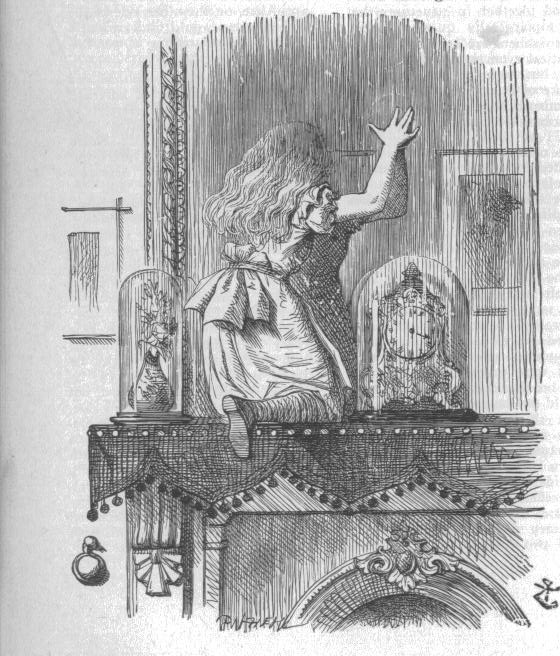
\includegraphics[width=\linewidth]{fig/intro/aliceroom.jpg}
	\caption{Looking glass room, by John Tenniel.}
\end{marginfigure}

\subsection{Conjunctive Queries}

We now turn to the $\textsf{query} \homto^? \textsf{data}$ side of the homomorphism problem. This perspective captures classical database evaluation and highlights how such queries naturally express existential, monotonic properties.
For instance, if $\?G$ is the "graph@@dir" with
two nodes $u$ and $v$ and a single edge from $u$ to $v$,
then asking if there is a "homomorphism" from $\?G$ to a graph $\?H$ amounts
to asking if there exists at least one edge in $\?G$.

As we would expect for any existential problem, they are monotonic:
if a solution exists, and we add more data, then a solution still exists.
More formally, for any "structure" $\?A$, $\?B$ and $\?B'$, if $\?B$ is a "substructure"
of $\?B'$ and $\?A \homto \?B$,
then $\?A \homto \?B'$.

The example of SQL queries (\Cref{ex:sql-as-hom}) is actually more than a mere example:
every "homomorphism problem" $\?A \homto \?B$ can be seen as a SQL query evaluation problem
where $\?A$ encodes a "query@@sem" in the \textsf{SELECT-WHERE-FROM}
fragment of SQL and $\?B$ is a relational database.
This fragment can also be characterized as the fragment
of "first-order logic" where universal quantification, union and negation are not allowed.
For instance, the SQL query of \Cref{ex:sql-as-hom} can be expressed by the formula
\begin{align*}
	\phi(\textsf{title}, \textsf{time}) \defeq\; 
	& \exists \textsf{movie\_id}.\, 
	\exists \textsf{length}.\, 
	\exists \textsf{director}.\,
	\exists \textsf{room\_id}.\, \\
	& \hphantom{\land~} \textsc{Movies}(\textsf{movie\_id}, \textsf{title}, \textsf{length}, \textsf{director}) \\
	& \land
	\textsc{Projections}(\textsf{movie\_id}, \textsf{room\_id}, \textsf{time}).
\end{align*} 
\begin{marginfigure}
	\centering
	\begin{tikzpicture}
		\node (a0) at (-.1,5.2) {};
		\node (a1) at (-.4,3.5) {};
		\node (a2) at (-.1,1.8) {};
		\node (a3) at (.1,1.8) {};
		\node (a4) at (.4,3.5) {};
		\node (a5) at (.1,5.2) {};

		\node (b0) at (-.2,5.2) {};
		\node (b1) at (-.8,3.1) {};
		\node (b2) at (-.5,1.5) {};
		\node (b3) at (-.4,.6) {};
		\node (b4) at (-.2,-.2) {};
		\node (b5) at (.2,-.2) {};
		\node (b6) at (.4,1) {};
		\node (b7) at (.2,1.4) {};
		\node (b8) at (-.5,2.6) {};
		\node (b9) at (-.4,3.8) {};
		\node (b10) at (.2,5.2) {};
	
		\draw[use Hobby shortcut, closed=true, draw=c2, fill=c2, fill opacity=.4] 
			(b0) .. (b1) .. (b2) .. (b3) .. (b4) .. (b5) .. (b6) .. (b7) .. (b8) .. (b9) .. (b10);
		\draw[use Hobby shortcut, closed=true, draw=c1, fill=c1, fill opacity=.4] 
			(a0) .. (a1) .. (a2) .. (a3) .. (a4) .. (a5);
		
		\node[vertex] at (0,5) (5) {};
		\node[vertex] at (0,4) (4) {};
		\node[vertex] at (0,3) (3) {};
		\node[vertex] at (0,2) (2) {};
		\node[vertex] at (0,1) (1) {};
		\node[vertex] at (0,0) (0) {};
		\node[font=\tiny, right=2em of 5] {\textsf{movie\_id}};
		\node[font=\tiny, right=2em of 4] {\textsf{title}};
		\node[font=\tiny, right=2em of 3] {\textsf{length}};
		\node[font=\tiny, right=2em of 2] {\textsf{director}};
		\node[font=\tiny, right=2em of 1] {\textsf{room\_id}};
		\node[font=\tiny, right=2em of 0] {\textsf{time}};

		\node[below= of 0] {output: \textsf{title}, \textsf{time}};
	\end{tikzpicture}
	\caption{
		\AP\label{fig:SQL-as-CQ}
		A "conjunctive query".
	}
\end{marginfigure}
Yet another characterization of these queries is as "conjunctive queries": such a "query@CQ"
consists of a "relational structure" together with a tuple of vertices, called ``"output@@var"''---this tuple
plays the same role as the \textsf{SELECT} statement in SQL.
For instance, the previous query can be expressed as the "conjunctive query"
of \Cref{fig:SQL-as-CQ}. The semantics of such a "query@CQ"
$\gamma = \tup{\?G, \bar x}$ is defined as follows:
given a relational database, seen as a "relational structure" $\?D$,
it returns every possible tuple $\bar d$ of elements of $\?D$ such that
there exists a "homomorphism" from $\?G$ to $\?D$ that sends $\bar x$ to $\bar d$.
Overall, these characterizations shows this fragment to be quite robust.

Hence, these problems boil down to
"homomorphism problems" of the form $\textsf{query} \homto^? \textsf{data}$.
Assuming that the "query@@sem" if fixed,
the naive algorithm to solve the "homomorphism problem"---consisting in enumerating
every possible function from $A$ to $B$ and checking whether some of them
define a "homomorphism"---works in polynomial time, as there are only $|B|^{|A|}$ such functions.
In fact, it is straightforward to devise an algorithm in "uniform-AC0"---actually, the depth
of the circuit does not even depend on $\?A$: there is roughly one layer simulating the
existential quantifiers, and another one simulating the conjunctions.

We now turn to the complexity of evaluating these "queries@CQ".
While $|B|^{|A|}$ is indeed polynomial when $\?A$ is fixed,
recall that $\?B$ represents a database:
even though complexity theory pretend that polynomial-time is tractable,
a polynomial-time algorithm of degree seven,
run over a 2.9 TB database, will execute more instructions
than there are atoms in the observable universe.
This leads to two natural questions:
\begin{itemize}
	\item optimizing the size of the exponent, "ie"
		replacing the "query@@sem" with a semantically equivalent one of smaller size,
	\item studying the parametrized complexity of the evaluating SQL queries, when parametrized by
		the size of the query. This provides a finer complexity notion than
		the classical "NP"/"AC0" approach; our previous remark shows the result to be
		slicewise polynomial ("XP"), which is not as well-behaved in practice than
		the "fixed-parameter tractable" ("FPT") problems.
\end{itemize}

\paragraph*{Query minimization.}
Both problems are in fact well-understood.
This problem of optimizing the \textsf{SELECT-WHERE-FROM} fragment of
SQL is well-understood, precisely by using the framework of "conjunctive queries"
and "relational structures".
This problem amounts to, given a "finite $\sigma$-structure" $\?A$,
deciding if there exists a strictly smaller "$\sigma$-structure" $\?A'$ "st",
for any "finite $\sigma$-structure" $\?B$, then
\[
	\?A \homto \?B
	\quad\text{"iff"}\quad
	\?A' \homto \?B.
\]
The property above is in fact equivalent to
\begin{equation}
	\?A \homto \?A'
	\quad\text{and}\quad
	\?A' \homto \?A
	\label{eq:intro-hom-equivalence}
\end{equation}
and is hence decidable.
The optimization procedure then goes as follows:
starting from $\?A$, we check for every possible vertex $a \in \?A$
if $\?A \smallsetminus \{a\}$ is equivalent to $\?A$ in the sense of
\Cref{eq:intro-hom-equivalence}. If some $a$ satisfy the property, we
let $\?A \smallsetminus \{a\}$ be our new query and start the process again.
Otherwise, we get a minimal "query@@CQ", called "core" of $\?A$.
This "core" is unique---which is not obvious since we defined it with
a greedy procedure---and is, by construction, a "substructure" of $\?A$.
In particular, it implies that the "core" does not only minimize the number of
vertices of $\?A$---while being "semantically equivalent"---, but also any
parameter that is closed under taking "substructures", such as "eg" the "tree-width".
Therefore, this notion of "core", together with seeing
\textsf{SELECT-WHERE-FROM} queries as "relational structures"/"conjunctive queries"
provides a remarkably robust tool for solving most optimization problem on these "queries@@CQ".

\begin{known}
	"Conjunctive queries" can be minimized by computing their "core".
	This process minimizes the number of vertices, but also many other
	parameters, such as "path-width", "tree-width", etc.
\end{known}

\paragraph*{FPT algorithms.}
The problem of whether a "graph@@undir" contains a "$k$-clique" easily reduces to a
"homomorphism problem" where the "input structure" is fixed---and equal to "$k$-clique".
It follows that the "homomorphism problem", parametrized in the
size of the "input structure" is "W1"-hard. Assuming that "W1" $\neq$ "FPT",%
\footnote{This is the parametrized counterpart of "P" $\neq$ "NP".}
it follows that there cannot be an "FPT" algorithm for evaluating "conjunctive queries".
This started a quest towards finding classes of "conjunctive queries" with an "FPT" evaluation.

\begin{marginfigure}
	\centering
	\begin{tikzpicture}
		\node[vertex] at (0,0) (eps) {};
		\node[vertex, below left=1.6em and 2em of eps] (a) {};
		\node[vertex, below right=1.6em and 2em of eps] (b) {};
		\node[vertex, below left=1.6em and 1.5em of a] (aa) {};
		\node[vertex, below=1.44em of a] (ab) {};
		\node[vertex, below right=1.6em and 1.5em of a] (ac) {};
		\node[vertex, below=1.44em of b] (ba) {};

		\draw[edge] (eps) to node[above left] {$\+R$} (a);
		\draw[edge] (eps) to node[above right] {$\+S$} (b);
		\draw[edge] (a) to node[above left] {$\+R$} (aa);
		\draw[edge] (a) to node[left] {$\+S$} (ab);
		\draw[edge] (a) to node[above right] {$\+T$} (ac);
		\draw[edge] (b) to node[right] {$\+R$} (ba);
	\end{tikzpicture}
	\caption{
		\AP\label{fig:intro-tree-shaped-CQ}
		A tree-shaped "conjunctive query" over a "signature"
		with three binary relations denoted by $a$, $b$ and $c$.
	}
\end{marginfigure}
First, one can notice that if said query is tree-shaped,
such as the "conjunctive query" of \Cref{fig:intro-tree-shaped-CQ}, then the naive
bottom-up evaluation algorithm works in time that is polynomial both
in the size of the query and in the size of the database.
Now, assume that $\gamma$ is a "conjunctive query" that is not necessarily
not tree-shaped, but that is equivalent to a tree-shaped "query@@CQ".
This is equivalent to saying that the "core" of $\gamma$ is "tree-shaped".
Hence, to evaluate $\gamma$, one can instead:
\begin{itemize}
	\item first compute its "core",
	\item then evaluate this "core" on the database.
\end{itemize}
The interest of this approach is that, while databases are ever-changing,
queries are often handwritten and somewhat short. Spending effort optimising them can be beneficial, since it might lead to performance gain
for \emph{every} evaluation of the query: this is why studying the
complexity of the evaluation problem parametrized by the size of
the query is relevant.
Formally, the previous procedure yields an algorithm that works in time
\[
	\+O(f(|\text{query}|) \cdot \text{poly}(|\text{core}|, |\text{database}|)).
\]
This means that evaluating "conjunctive queries" that are semantically equivalent to
tree-shaped "queries@CQ" is "FPT".

In fact, for this reasoning to work, the notion of ``tree-shaped'' need not
be as restrictive as what is shown in \Cref{fig:SQL-as-CQ}: for instance,
edges could be reversed. More generally, if the "query@@CQ" has "tree-width"%
\footnote{Tree-width is a graph-parameter that measure how far a graph is from a tree.
The notion can be extended to "relational structures".}
at most $k$, then we still get a polynomial-time evaluation algorithm---where the order
of the polynomial depends on $k$. In turns, it means that for every $k\in\Np$,
evaluating "conjunctive queries" that are semantically equivalent to
a "queries@CQ" of "tree-width" at most $k$ is "FPT".\footnote{In fact,
they can even be evaluated in polynomial time, but the argument is less straightforward
\cite{ChekuriRajaraman2000TreeWidthPolytime}.}

Remarkably, this is \emph{exactly} the limit of tractability for these "queries@CQ":
Grohe showed that a class of "conjunctive queries"
satisfying mild closure properties has "FPT" evaluation "iff"
it has bounded ``"semantic tree-width"''---meaning that there exists $k\in\Np$ "st"
every "query@CQ" in the class is "semantically equivalent" to a "query@CQ" 
of "tree-width" at most $k$ \cite{Grohe2007ComplexityHomomorphism}.%
\footnote{The same equivalent holds for polynomial-time evaluation.}

\begin{known}
	"Conjunctive queries" of bounded semantic tree-width are exactly
	the classes of "conjunctive queries" with tractable evaluation.
\end{known}


\subsection{Beyond Conjunctive Queries: Adding Regular Path Predicates for Human-Centered Data}

\begin{marginfigure}
	\centering
	\begin{tikzpicture}
		\node[vertex] at (0,2) (2) {};
		\node[vertex] at (0,1) (1) {};
		\node[vertex] at (0,0) (0) {};

		\draw[edge] (0) to (1);
		\draw[edge] (1) to (2);

		\node[font=\tiny, right=0em of 2] {\textsf{person}};
		\node[font=\tiny, right=0em of 1] {\textsf{child}};
		\node[font=\tiny, right=0em of 0] {\textsf{grand\_child}};

		\node[below= of 0] {output: \textsf{person}, \textsf{grand\_child}};
	\end{tikzpicture}
	\caption{
		\AP\label{fig:CQ-grandchild}
		A "conjunctive query" outputting all pairs of people with their grandchildren.
	}
\end{marginfigure}
Overall, the theory of \emph{conjunctive queries} is hence well-understood.
Even when considering other features from SQL, such as aggregate functions---\textsf{COUNT}, \textsf{SUM}, etc.---, the query language of "conjunctive queries" faces a big limitation:
it is \emph{intrinsically local}.
Consider two "structures" $\?A$ and $\?B$, and two elements $a$ and $a'$ of $A$.
For any homomorphism $f$ from $\?A$ to $\?B$, the "distance@@struct" from $f(a)$ to $f(a')$
in $\?B$ is at most the distance from $a$ to $a'$ in $\?A$.\footnote{This follows from
the definition of a "homomorphism", by using a trivial induction on the "distance@@struct".}
Now assume that $\?B$ is a "graph@@dir", whose vertices are humans,
and whose edges represent the `is a child of' relation.
For any $k\in\N$, it is easy to build a "conjunctive query" $\tup{\?A_k, \tup{a, a'}}$
outputting all pairs $\tup{b,b'}$ "st" $b'$ is a depth-$k$ descendant of $b$---see
\Cref{fig:CQ-grandchild} for $k=2$.
However, since "homomorphisms" contract "distances@@struct", there is no
"conjunctive query" $\tup{\?A_*, \tup{a, a'}}$ outputting all pairs $\tup{b,b'}$
"st" $b'$ is descendant, at \emph{any} depth, of $b$.
In other words, "conjunctive queries" are not closed under transitive closures.

More generally, human-centered data does not usually go well with
relational databases, as they are not designed to allow graph traversal.
To face this issue, "graph databases", also known as "knowledge graph" have
been introduced: they can essentially be modelled
as "relational structures" whose relations are all binary, "ie"
as edge-labelled graphs---see "eg" \Cref{fig:example-wikidata}.
To illustrate this point, we consider
"Wikidata", which is a knowledge graph containing more than one hundred million
vertices, whose data is used amongst others on Wikipedia. 
We would like to obtain all literary works published before 1990 and whose
French title contains the string ``exist''.
This can be done using the SPARQL query language, which is roughtly the equivalent
of SQL for knowledge bases: the query is represented in \Cref{fig:sparql,fig:sparql-explained}.
\begin{figure}
\lstinputlisting[language=SQL, morekeywords={rdfs,wd,wdt,FILTER,LANG,CONTAINS}]{fig/intro/exist.rq}
	\caption{
		\label{fig:sparql}
		A SPARQL query.\\
	\href{https://query.wikidata.org/\#SELECT\%20DISTINCT\%20\%3Fwork\%20\%3FworkLabel\%20\%3FauthorLabel\%0AWHERE\%0A\%7B\%0A\%20\%20\%3Fwork\%09wdt\%3AP31\%2Fwdt\%3AP279\%2a\%20wd\%3AQ7725634\%3B\%0A\%20\%20\%20\%20\%20\%20\%20\%20rdfs\%3Alabel\%20\%3FworkLabel\%3B\%0A\%20\%20\%09\%09wdt\%3AP577\%20\%3Fdate\%3B\%0A\%20\%20\%20\%20\%20\%20\%20\%20wdt\%3AP50\%20\%3Fauthor.\%0A\%20\%20\%3Fauthor\%20rdfs\%3Alabel\%20\%3FauthorLabel.\%0A\%20\%20FILTER\%28LANG\%28\%3FworkLabel\%29\%20\%3D\%20\%22fr\%22\%20\%26\%26\%20LANG\%28\%3FauthorLabel\%29\%20\%3D\%20\%22fr\%22\%29.\%0A\%20\%20FILTER\%28CONTAINS\%28\%3FworkLabel\%2C\%20\%22exist\%22\%29\%29.\%0A\%20\%20FILTER\%28YEAR\%28\%3Fdate\%29\%20\%3C\%3D\%201990\%29.\%0A\%7D\%0ALIMIT\%207}{[\raisebox{-.4ex}{\HandRight} Execute the query.]}
	}
\end{figure}
\begin{figure}
	\lstinputlisting[language=SQL, morekeywords={rdfs,wd,wdt,FILTER,LANG,CONTAINS}]{fig/intro/exist-bis.txt}
	\caption{
		\label{fig:sparql-explained}
		Human-friendly translation of the SPARQL query of \Cref{fig:sparql}.
	}
\end{figure}
The central notion in knowledge graphs and SPARQL is the notion of triplets:
\lstinline[language=SQL]{x R y.} refers to an edge of the \textsf{R}-relation
going from \textsf{x} to \textsf{y}.
Then \lstinline[language=SQL]{x R y; S z.} is an abbreviation for
\lstinline[language=SQL]{x R y. x S z.}
Hence, the central part (ll.~4--8) of the SPARQL query of \Cref{fig:sparql,fig:sparql-explained}
should be understood as follows:
we are looking for variables \textsf{?work}, \textsf{?typeOfWork} (implicit),
\textsf{?workLabel}, \textsf{?date} and \textsf{?authorLabel} "st":
\begin{itemize}
	\item there is a path from \textsf{?work} to \textsf{?typeOfWork}
		obtained by taking an edge `is instance of', and then an arbitrary number
		of edges of type `is subclass of',
	\item \textsf{?typeOfWork} should exactly correspond to the vertex called `type of work',
	\item \textsf{?work} has label \textsf{?workLabel}, 
	\item \textsf{?work} was published on \textsf{?date},
	\item \textsf{?work} was authored by \textsf{?author}, and
	\item \textsf{?author} has label \textsf{?authorLabel}.
\end{itemize}
They key feature of graph databases query languages is illustrated
with the \lstinline[language=SQL]{wdt : P31 / wdt : P279 *}:
this expression does not refer to a single edge of the knowledge graph,
but rather to a regular expression formed from these edges.
These regular expressions are precisely what allows for easy graph traversal!
An example of a match of this expression is provided
in red in \Cref{fig:example-wikidata}.
The output of the query of \Cref{fig:sparql,fig:sparql-explained}
is provided in \Cref{tab:output-sparql}.

\begin{figure}
	\centering
	\begin{tikzpicture}
		\node[vertex] at (0,-.5) (stats) {};
		\node[vertex] at (-1.5,-1.5) (FF) {};
		\node[vertex] at (0,-2.1) (1892) {};
		\node[vertex] at (1.5,-1.5) (French) {};
		\node[vertex] at (0,1) (bioDic) {};
		\node[vertex] at (-1.5,2) (bio) {};
		\node[vertex] at (0,2) (dico) {};
		\node[vertex] at (1.5,2) (cata) {};
		\node[vertex] at (.5,3) (kl) {};
		\node[vertex] at (-.5,3) (ref) {};
		\node[vertex] at (-1.5,3) (bioW) {};
		\node[vertex] at (-1.5,4) (nonFic) {};
		\node[vertex] at (1.5,3) (lit) {};

		\draw[edge] (stats) to node[fill=white, midway, font=\tiny] {author} (FF);
		\draw[edge] (stats) to node[fill=white, midway, font=\tiny] {date} (1892);
		\draw[edge] (stats) to node[fill=white, midway, font=\tiny] {language} (French);
		\draw[edge, draw=c0] (stats) to node[fill=white, midway, font=\tiny, text=c0] {instance of} (bioDic);

		\draw[edge, bend left, dotted] (bioDic) to (bio);
		\draw[edge, bend right, dotted] (bioDic) to (cata);
		\draw[edge, dotted, draw=c0] (bioDic) to (dico);

		\draw[edge, dotted] (bio) to (bioW);
		\draw[edge, dotted] (bioW) to (nonFic);
		\draw[edge, dotted] (cata) to (ref);
		\draw[edge, dotted] (cata) to (kl);
		\draw[edge, dotted] (dico) to (kl);
		\draw[edge, dotted] (dico) to (ref);
		\draw[edge, dotted, draw=c0] (dico) to (lit);

		\node[right=1em of stats, font=\tiny, color=cDarkGrey, text width=3.5cm]
			{"Statistique des gens de lettres et des savants existant en France@@wd"};
		\node[below left=-.25em of FF, font=\tiny, color=cDarkGrey, text width=2cm, align=right]
			{"François-Fortuné Guyot de Fère@@wd"};
		\node[below=-.25em of 1892, font=\tiny, color=cDarkGrey]
			{1892};
		\node[below right=-.25em of French, font=\tiny, color=cDarkGrey]
			{"French@@wd"};
		\node[below left=-.5em and 1em of bioDic, font=\tiny, color=cDarkGrey, text width=1.5cm, align=right]
			{"biographical dictionary@@wd"};
		\node[left=-.25em of bio, font=\tiny, color=cDarkGrey]
			{"biography@@wd"};
		\node[below right=-.25em and -.25em of dico, font=\tiny, color=cDarkGrey]
			{"dictionary@@wd"};
		\node[right=-.25em of cata, font=\tiny, color=cDarkGrey]
			{"catalogue@@wd"};
		\node[above=.25em of kl, font=\tiny, color=cDarkGrey, text width=2cm, align=center]
			{"knowledge organization system@@wd"};
		\node[above=-.25em of ref, font=\tiny, color=cDarkGrey]
			{"reference work@@wd"};
		\node[left=-.25em of bioW, font=\tiny, color=cDarkGrey]
			{"biographical work@@wd"};
		\node[left=-.25em of nonFic, font=\tiny, color=cDarkGrey]
			{"non-fiction work@@wd"};
		\node[right=-.25em of lit, font=\tiny, color=cDarkGrey]
			{"literary work@@wd"};
	\end{tikzpicture}
	\caption{
		\AP\label{fig:example-wikidata}
		Part of the "Wikidata" knowledge graph.
		Dotted arrows represent the relation `subclass of'.
		The red path matches the expression \lstinline[language=SQL]{wdt : P31 / wdt : P279 *}.
		For readability, labels are written next to the vertices
		rather than as separate vertices linked with a `has label' relation.
	}
\end{figure}
\begin{table}
	\centering
	{
		\footnotesize%
		\begin{tabular}{ll}
			\toprule
			workLabel & authorLabel \\ \midrule 
			Statistique des gens de lettres 
				& \multirow{2}{*}{François-Fortuné Guyot de Fère}\\
			et des savants existant en France
				& \\
			Le Chevalier inexistant
				& Italo Calvino\\
			L'existentialisme est un humanisme
				& Jean-Paul Sartre\\
			Ennui existentiel
				& Anton Tchekhov\\
			Les Ennuis de l'existence
				& Anton Tchekhov\\
			La tentation d'exister
				& Emil Cioran\\
			Inexistence
				& David Zindell \\ \bottomrule
		\end{tabular}
	}
	\caption{
		\AP\label{tab:output-sparql}
		Output of the SPARQL query of \Cref{fig:sparql,fig:sparql-explained}.}
\end{table}

We formalize the core features of SPARQL as "conjunctive regular path queries":
they consist of "conjunctive queries", except that their atoms are no
longer of the form $x \atom{\+R} y$ (for some binary relation $\+R \in \sigma$),
but can be more generally of the form
\[
	x \atom{L} y
	\quad\text{ for some "regular language" $L$ over $\sigma$}.
\]
For instance, ll.~1--8 of the SPARQL query of \Cref{fig:sparql,fig:sparql-explained}
can be modelled by the "conjunctive regular path query" of \Cref{fig:intro-SPARQL-as-CRPQ}:
notice the regular expression in red.
\begin{marginfigure}
	\centering
	\begin{tikzpicture}
		\node[vertex] at (0,0) (work) {};
		\node[vertex, above=3em of work] (litWork) {};
		\node[vertex, below left=2.2em and 2.7em of work] (workLabel) {};
		\node[vertex, below=2.9em of work] (date) {};
		\node[vertex, below right=2.2em and 2.7em of work] (author) {};
		\node[vertex, below=2.5em of author] (authorLabel) {};

		\draw[edge] (work) to node[fill=white, font=\tiny, text=c0] {instance $\cdot$ subclass${}^*$} (litWork);
		\draw[edge] (work) to node[fill=white, font=\tiny] {label} (workLabel);
		\draw[edge] (work) to node[fill=white, font=\tiny] {date} (date);
		\draw[edge] (work) to node[fill=white, font=\tiny] {author} (author);
		\draw[edge] (author) to node[fill=white, font=\tiny] {label} (authorLabel);

		\node[right=-.25em of work, font=\tiny, color=cDarkGrey]
			{work};
		\node[right=-.25em of litWork, font=\tiny, color=cDarkGrey]
			{typeOfWork};
		\node[left=-.25em of workLabel, font=\tiny, color=cDarkGrey]
			{workLabel};
		\node[below=-.25em of date, font=\tiny, color=cDarkGrey]
			{date};
		\node[right=-.25em of author, font=\tiny, color=cDarkGrey]
			{author};
		\node[right=-.25em of authorLabel, font=\tiny, color=cDarkGrey]
			{authorLabel};

		\node[below=4.5em of date] {output: \textsf{workLabel}, \textsf{authorLabel}};
	\end{tikzpicture}
	\caption{
		\AP\label{fig:intro-SPARQL-as-CRPQ}
		A "conjunctive regular path query" 
		modelling the core part of \Cref{fig:sparql,fig:sparql-explained}.
	}
\end{marginfigure}

\begin{known}
	"Graph databases"/knowledge graphs store information as edge-labelled graphs.
	To allow for graph traversal, we extend "conjunctive queries"
	to "conjunctive regular path queries" by adding regular expressions.
\end{known}


\subsection{Minimization and Structure of Conjunctive Regular Path Queries}

While "conjunctive regular path queries" share some enjoyable properties
of "conjunctive queries"---for instance the decidability of "semantical equivalence",
in contrast to "eg" "first-order logic"---its semantics is more complex:
graph-like phenomenon ("homomorphisms") intertwines with "regular languages".
Not only does this lead to a complexity blow-up---"semantical equivalence" is "NP"-complete
for "conjunctive queries" but "ExpSpace"-complete for "conjunctive regular path queries"---,
it also breaks the nice theory of "cores".

As a consequence, the optimizing "conjunctive regular path queries" poses
a significant challenge to untwist graph properties from automata-theoretic ones.
This first part of this thesis is dedicated to this problem.
After exposing the basic theory of "conjunctive regular path queries"
in \Cref{ch:prelim-graph-databases}, we study
the "minimization problem@@CRPQ" in \Cref{ch:minimization-CRPQ}:
given such a "query@CRPQ" and $k\in\Np$, we can decide if it is equivalent to a "query@CRPQ"
of size at most $k$, and if so we can produce it.

\begin{contribution}
	Whether a "conjunctive regular path query" can be minimized is decidable,
	and minimization is effective.
\end{contribution}

We notice that, somewhat unexpectedly, there are some "conjunctive regular path queries"
that are minimal in the sense above, but that are equivalent to a \emph{finite union}---in the 
semantical sense---of strictly smaller "conjunctive regular path queries".%
\footnote{This contrasts with the case of "conjunctive queries",
where the notion of "core" and the order-theoretic properties
of "relational structures" precisely prevents this phenomenon from appearing.
In other words, this phenomenon precisely emerges by interlacing
the graph structure and the automata of the "query@@CRPQ".}
We argue that measuring a union of such "queries@@CRPQ" by the maximal size
of a query in the union is a sensitive thing to do---because the complexity
of evaluating such a union depends mostly on this parameter---, and prove
that given a "conjunctive regular path queries" and $k\in\N$, we can
decide if it is equivalent to a finite union of
"queries@CRPQ" which are all of size at most $k$.

\begin{contribution}
	Whether a "conjunctive regular path query" can be minimized
	as a union of strictly smaller "queries@@CRPQ" is decidable,
	and minimization is effective.
\end{contribution}

Both algorithms are essentially brute-force, and the main technical difficulty
lies in proving that finitely many candidates to test, which is not
trivial because we do not ask for any bound on the size of the "regular languages".%
\footnote{Again, the motivation lies from the fact that the complexity of evaluating
a "conjunctive regular path queries" mostly depends on how many "atoms"/edges it has,
and not so much on how complex these languages are.}
The idea behind the two algorithms are in fact surprisingly different:
\begin{itemize}
	\item in the first case---when union is not allowed---, we prove that
		if a "query@CRPQ" is equivalent to another one with few
		"atoms" (but potentially big languages), then it must be
		equivalent to a "query@CRPQ" with few "atoms" \emph{and} small languages.
		This property is proved by understanding the subtle interactions between
		languages and the graph structure;
	\item in the second case---when union is allowed---, we build a canonical
		finite union of "queries@CRPQ", corresponding to the
		"maximal under approximation" by a finite union of small "queries@CRPQ": 
		it is the \emph{best} under approximation---in the sense that
		it logically entails the "query@CRPQ"---and so, if the original
		"query@CRPQ" is equivalent to a finite union of small ones, then
		it must be equivalent to this "maximal under approximation".
		The difficulty there lies in proving the existence of "maximal under approximation",
		or rather that it can be expressed by a \emph{finite} union.
		This construction can essentially be seen as a
		smart brute-forcing, obtained by agglomerating all possible smaller "queries@CRPQ".
\end{itemize}

One reason we resolve to using brute-force algorithm is that it is
remarkably hard to understand when a "query@CRPQ" cannot be minimized.
The case of "conjunctive queries" is much simpler: if the "core" 
of the "query@CQ" has $k$ edges (resp. "tree-width" $k$),
then any "conjunctive query" "semantically equivalent" to it must use at least $k$ edges
(resp. have "tree-width" at least $k$).
Another of our contributions is to identify a sufficient condition%
\footnote{However, contrary to the "core", this condition is not necessary.}
on a "query@CRPQ" so that \emph{any} "query" "semantically equivalent" to it
must contain a ``complex pattern''. The strength of this theorem lies in its
general applicability, as the notion of ``complex pattern''
is formalized as a ``"minor-closed" class
of graphs''---examples include the class of all graphs with at most $k$ "atoms",
or the class of all graphs of "tree-width" at most $k$.

\begin{contribution}
	We introduce the "semantical structure theorem", that provides
	a way to prove lower bounds on the number
	of "atoms", or "tree-width", or any minor-closed property,
	that is necessary to express a "query@@sem".
\end{contribution}

This tool proves useful to prove minimality of specific examples---"ie"
for proofs---, and to prove complexity lower bounds for our problem.
However, this it only provides a sufficient condition, that is often not
necessary, it fails to provide a \emph{simple} algorithm to test minimality---hence our
brute-force algorithms.

Then, in \Cref{ch:semantic-tree-width-CRPQ}, we turn to the question
of "tree-width". Similarly to "conjunctive queries", finite unions of
"conjunctive regular path queries"
of bounded "tree-width" can be evaluated in polynomial time.
It begs the question of deciding when a "query@CRPQ" is actually equivalent
to such an object.

\begin{known}
	Barceló, Romero and Vardi \cite{BarceloRomeroVardi2016SemanticAcyclicity}
	devised an algorithm to test
	if a "conjunctive regular path queries" is equivalent to
	a finite union of ``acyclic''---meaning of "tree-width" 1---"queries@CRPQ".
\end{known}

Unfortunately, the general question for "tree-width" $k$ is left open at the end
of their paper as the authors did not know how to extend their technique to this
more general setting. We extend their result, relying again on the notion
of "maximal under-approximation":%
\footnote{The paper of Barceló, Romero and Vardi
also relies on "maximal under-approximations", and this notion already existed
for "conjunctive queries".}
we prove that, given a "conjunctive regular path query" and
$k\in\Np$ the existence and computability of its "maximal under-approximation"
by finite unions of "queries@CRPQ" of "tree-width" at most $k$.

\begin{contribution}
	Given $k\in \Np$ and a "conjunctive regular path queries",
	we can decide if the latter is "semantically equivalent"
	to a finite union of "queries@CRPQ" of "tree-width"
	(resp. "path-width") at most $k$.
\end{contribution}

The proof of existence of this "maximal under-approximation" is
actually quite hard---at least much harder than in the case minimizing
the number of "atoms"---as it needs to deal with two kind of information:
the structure of the query, "ie" its underlying graph, and its languages.
The proof precisely massages the query to, at the same time,
preserve information about the "tree decomposition"---serving as a
witness of the small "tree-width" of the "query@CRPQ"---and about the
semantics of the "query@CRPQ".

Amusingly, we originally thought that our proof was not able to
capture the case $k=1$ that was already handled, and that the constructions
of Barceló, Romero and Vardi and ours were orthogonal.
When written the journal version of this paper---that was originally
published at ICDT '23---, we wanted to extend the results to "path-width",%
\footnote{The main motivation behind this is that the evaluation of "queries@CRPQ"
of bounded "path-width" is not only polynomial but even "NL"!}
but part of our construction broke. Introducing the technical tool
to fix it\footnote{See the notions of "contractions" and "contracted path-width".}
actually leads to a unified solution, that handles both
the case of "tree-width" $k$ (including $k=1$) and "path-width".%
\footnote{Lastly, note that the order of presentation of these results
does not follow the timeline of their discovery: our work on "semantic tree-width"
was done in 2022--23 and published at ICDT '23, while the one on minimization
was done in 2024--25 and published at PODS '25.}

Lastly, all these algorithms relies on testing the equivalence
of "conjunctive regular path queries", which is "ExpSpace".
It leads to resource-hungry algorithms,%
\footnote{Although it has to be noted that it is worth running exponential
algorithm on smallish "queries@CRPQ" in order to optimize
its evaluation on huge databases!}
which leads to a natural quest for identifying subclasses
of "queries@CRPQ" that admit more efficient algorithms.

"Conjunctive regular path queries" over "simple regular expression",
where the "regular languages" allowed are restricted to be concatenations of
edge-labels and reflexive-transitive closure ("aka" Kleene star) of
edge-labels, were already known to have a more efficient
algorithm for testing "semantical equivalence".

\begin{contribution}
	We prove that the problem of minimizing the number of "atoms" (resp. "tree-width")
	of "conjunctive regular path queries" over "simple regular expression"
	lies in the polynomial hierarchy.
\end{contribution}

A consequence of our work on "tree-width" is that,
given a "conjunctive regular path query" that is promised to be equivalent
to a "query@CPRQ" of "tree-width" $k$, we can first compute said
equivalent query of small "tree-width" by using our algorithm,
and then evaluate it on any database. This proves that the evaluation
problem for "conjunctive regular path queries" of bounded "semantic tree-width"
is "FPT" when parametrized by the size of the "query@@sem".%
\footnote{This result was in fact already known---but proven differently, with
an incomparable complexity (better preprocessing but worst polynomial exponent)---by
Romero, Barceló and Vardi \cite{RomeroBarceloVardi2017Homomorphism}.}

Whether the converse hold remains a mystery: many attempts
have been tried to extend Grohe's proof for "conjunctive queries" to this setting,
but all failed, precisely because of the difficulty posed
by the intertwining of the graph structure and the automata.
We conclude this part of the thesis by a discussion of this problem,
as well as whimsical ideas related to "conjunctive regular path queries"
in \Cref{ch:conclu-database}.

\begin{openproblemintro}
	Characterize the "classes of CRPQ" with "FPT" evaluation
	when parametrized in the size of the "query@CRPQ".
\end{openproblemintro}

To summarize, the $\textsf{query} \homto^? \textsf{data}$ formulation of the "homomorphism problem" provides a robust foundation for classical database theory. The first part of this thesis extends this framework to a richer context: graph databases and queries extended with regular path predicates.
\section{Everyone Who Wants to Do Constraint Satisfaction Always Ends in Universal Problems}
% Everyone who wants to do good to the human race always ends in universal bullying.
% - Aldous Huxley
\label{sec:intro-universal}

\subsection{Constraint Satisfaction Problems}

This second part explores the complexity of the "homomorphism problem" when the data is fixed and the query varies, focusing on "constraint satisfaction problems" and "automatic structures".

\begin{marginfigure}[-15em]
	\centering
	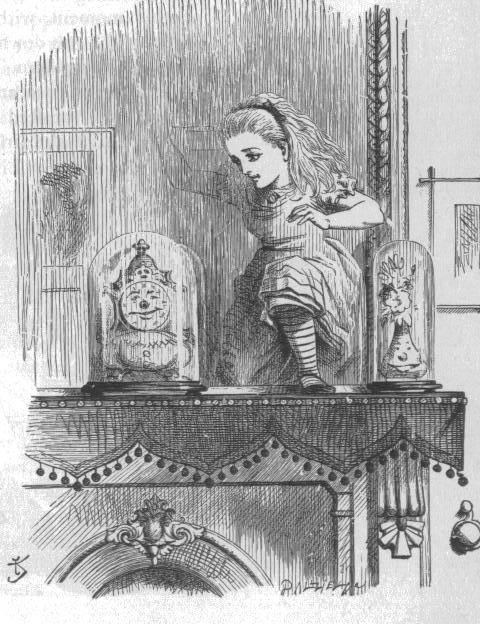
\includegraphics[width=\linewidth]{fig/intro/aliceroom2.jpg}
	\caption{Looking glass room, by John Tenniel.}
\end{marginfigure}

\paragraph*{Constraint Satisfaction Problems.}
Going to the other side, encodings of model-checking problems
as "homomorphism problems" of the form $\textsf{data} \homto^? \textsf{query}$
can be thought of as ``universal problems''---here ``universal'' does not
refer to some form of completeness, but simply to universal quantification.
Notice "eg" that they are anti-monotonic with respect to the data:
for all "structures" $\?A$, $\?A'$ and $\?B$, if $\?A \homto \?B$ and $\?A'$ is a substructure
of $\?A$ then $\?A' \homto \?B$.
Moreover, while problems of the form $\textsf{query} \homto^? \textsf{data}$
can be solved locally---whether a vertex of the data is part of a solution (a "homomorphism") only 
depends on its "neighbourhood"---, problems of type $\textsf{data} \homto^? \textsf{query}$ cannot.

\begin{marginfigure}[-18em]
	\centering
	\begin{tikzpicture}
		% ---
% 3-clique
% ---
\node[vertex, draw=c0, fill=c0, fill opacity=.4] at (0,0) (k3-0) {};
\node[vertex, above right=1em and 2em of k3-0, draw=c1, fill=c1, fill opacity=.4] (k3-1) {};
\node[vertex, below right=1em and 2em of k3-0, draw=c2, fill=c2, fill opacity=.4] (k3-2) {};

\draw[edge, bend right=15] (k3-0) to (k3-1);
\draw[edge, bend right=15] (k3-0) to (k3-2);
\draw[edge, bend right=15] (k3-1) to (k3-0);
\draw[edge, bend right=15] (k3-1) to (k3-2);
\draw[edge, bend right=15] (k3-2) to (k3-0);
\draw[edge, bend right=15] (k3-2) to (k3-1);
	\end{tikzpicture}
	\caption{
		\AP\label{fig:intro-3-clique}
		The "$3$-clique" $\clique{3}$.
	}
\end{marginfigure}
\begin{marginfigure}[-6em]
	\centering
	\begin{tikzpicture}
		% ---
% Example 3-colouring
% ---
\tikzset{every node/.style={fill opacity=.4}}
\node[vertex, color=c0, fill=c0] at (0,0) (0) {};
\node[vertex, above left=.75em of 0, color=c1, fill=c1] (0al) {};
\node[vertex, above right=.75em of 0, color=c2, fill=c2] (0ar) {};
\node[vertex, below left=2em of 0al, color=c0, fill=c0] (0l) {};
\node[vertex, below right=2em of 0ar, color=c0, fill=c0] (0r) {};
\node[vertex, above left=of 0l, color=c1, fill=c1] (0ll) {};
\node[vertex, above right=of 0r, color=c2, fill=c2] (0rr) {};
\node[vertex, below left=of 0, color=c2, fill=c2] (0bl) {};
\node[vertex, below right=of 0, color=c1, fill=c1] (0br) {};

\node[vertex, below=2em of 0, color=c0, fill=c0] (1) {};
\node[vertex, below left=1em of 1, color=c1, fill=c1] (1bl) {};
\node[vertex, below right=1em of 1, color=c2, fill=c2] (1br) {};
\node[vertex, above left=0em and 1.5em of 1bl, color=c2, fill=c2] (1bll) {};
\node[vertex, above right=0em and 1.5em of 1br, color=c1, fill=c1] (1brr) {};

\node[vertex, below=4em of 1, color=c0, fill=c0] (2) {};
\node[vertex, below left=1.5em and .75em of 1bl, color=c2, fill=c2] (2al) {};
\node[vertex, below right=1.5em and .75em of 1br, color=c1, fill=c1] (2ar) {};
\node[vertex, below left=.5em and 1.5em of 2, color=c1, fill=c1] (2bl) {};
\node[vertex, below right=.5em and 1.5em of 2, color=c2, fill=c2] (2br) {};
\node[vertex, below left=of 2al, color=c0, fill=c0] (2ll) {};
\node[vertex, below right=of 2ar, color=c0, fill=c0] (2rr) {};

\draw[edge] (0) to (0al);
\draw[edge] (0) to (0ar);

\draw[edge] (0al) to (0l);
\draw[edge] (0l) to (0bl);
\draw[edge] (0bl) to (0);
\draw[edge] (0l) to (0ll);

\draw[edge] (0ar) to (0r);
\draw[edge] (0r) to (0br);
\draw[edge] (0br) to (0);
\draw[edge] (0r) to (0rr);

\draw[edge] (0bl) to (1);
\draw[edge] (1) to (1bl);
\draw[edge] (1bl) to (0l);

\draw[edge] (0br) to (1);
\draw[edge] (1) to (1br);
\draw[edge] (1br) to (0r);

\draw[edge] (1bl) to (2al);
\draw[edge] (2al) to (2ll);
\draw[edge] (2) to (2al);
\draw[edge] (2) to (2bl);
\draw[edge] (2bl) to (2al);

\draw[edge] (1br) to (2ar);
\draw[edge] (2ar) to (2rr);
\draw[edge] (2) to (2ar);
\draw[edge] (2) to (2br);
\draw[edge] (2br) to (2ar);

\draw[edge] (1bl) to (1bll);
\draw[edge] (1br) to (1brr);

\draw[edge, bend right=20] (2) to (1bl);
\draw[edge, bend left=20] (2) to (1br);


	\end{tikzpicture}
	\caption{
		\AP\label{fig:dichotomy-ex-3-clique}
		A "$3$-colouring" of some beetle-shaped "graph@@dir".
	}
\end{marginfigure}
\begin{example}[Graph colouring]
	\AP\label{ex:graph-colouring-as-hom}
	Let $k\in\Np$. We let the \AP""$k$-clique"", denoted by $\intro*\clique{k}$,
	to be the "graph@@dir" whose vertices are $\lBrack 1,k\rBrack$,
	and with an edge from $i$ to $j$ (with $i,j \in \lBrack 1,k\rBrack$)
	"iff" $i\neq j$, see \Cref{fig:intro-3-clique}.
	We say that a finite "graph@@dir" $\?G$ is \AP""$k$-colourable"" when
	we can map every vertex of $\?G$ to an element of $\lBrack 1,k\rBrack$
	"st" no two adjacent vertices are sent on the same colour/number.
	In other words, a $k$-colouring corresponds precisely to a "homomorphism" from $\?G$
	to $\clique{k}$, where colours correspond to the vertices of the clique,
	see "eg" \Cref{fig:dichotomy-ex-3-clique}.
	Hence, a graph is "$k$-colourable" if, and only if,
	there is a "homomorphism" from $\?G$ to $\clique{k}$.
\end{example}

For instance, "$3$-colourability" is a global property of a graph and cannot be solved
by gluing local solutions. In particular, this implies that fixing the query
does not necessarily result in
a drop in the complexity: "$3$-colourability" is already "NP"-complete!
The next example shows that, even when the "target structure" is fixed, the "homomorphism problem"
provides a flexible framework to encode problems.

\begin{example}[SAT solving]
	\AP\label{ex:sat-as-hom}
	We consider a 3-SAT instance, namely a finite conjunction of
	disjunctions of three literals, say
	\[
		\phi \defeq \bigwedge_{i=1}^n \ell_{i,1} \lor \ell_{i,2} \lor \ell_{i,3},
	\]
	where each $\ell_{i,j}$ is either a variable, or the negation of a variable.
	We assume "wlog" that in each clause, positive variables appear before negative ones:
	this of course can be achieved by a simple syntactical rewriting of each clause.%
	\footnote{Meaning "eg" that $x \lor \neg y \lor z$ is not allowed, contrary to
	$x \lor z \lor \neg y$.}
	We let $\?B$ be the structure whose domain has two elements $\{0,1\}$,
	equipped with four ternary relations $\+R_0$ through $\+R_3$, where $\+R_j$ encodes clauses with exactly $j$ negated literals. They are formally defined as
	\begin{align*}
		\+R_0 & \defeq \set{0,1}^3 \smallsetminus \set{\tup{0,0,0}}, &
		\+R_1 & \defeq \set{0,1}^3 \smallsetminus \set{\tup{1,0,0}}, \\
		\+R_2 & \defeq \set{0,1}^3 \smallsetminus \set{\tup{1,1,0}} \qquad\text{ and} &
		\+R_3 & \defeq \set{0,1}^3 \smallsetminus \set{\tup{1,1,1}}.
	\end{align*}
	We then encode $\phi$ into the "relational structure" $\?F_\phi$
	whose domain is the set of variables of $\phi$,
	and for every $i \in \lBrack 1,n \rBrack$,
	$\+R_j$ ($j\in\lBrack 0,3\rBrack$) consists of all triplets of variables $\tup{x,y,z}$
	"st" there is a clause of $\phi$ containing variables $x$, $y$ and $z$ (with multiplicity), and exactly $j$ of these variables occur negatively.
	For instance, $\tup{x, y, \neg x} \in \+R_1$, and $\tup{\neg x, \neg y, \neg z} \in \+R_3$.
	A function $f$ from the domain of $\?F_\phi$ to the domain of $\?B$ amounts to picking
	a Boolean valuation of the variables occurring in $\phi$.
	Observe that, by definition of the relations $\+R_j$,
	given a clause $\psi$ containing variables $x,y,z$, 
	$f$ is a "homomorphism" from $\?F_\psi$ to $\?B$ "iff"
	$f$, seen as a valuation, satisfies $\psi$.\footnote{For instance,
	if all variables are positive, then all valuations except the one putting
	all variables to false satisfy the formula. This is why $\+R_0$ is defined
	on $\?B$ as $\set{0,1}^3\smallsetminus \set{\tup{0,0,0}}$.}
	By taking conjunction, the conclusion follows: "homomorphisms" from
	$\?F_\phi$ to $\?B$ exactly correspond to valuations satisfying $\phi$.
	In particular, there is a "homomorphism" from $\?F_\phi$ to $\?B$ "iff"
	$\phi$ is satisfiable.%
	\footnote{Note that this example can be easily generalized to $k$-SAT for any $k\in\Np$.
	However, the "signature" depends on $k$.}
\end{example}

However, contrary to "$3$-colourability" and SAT solving, not all of these problems are NP-hard. For example, $2$-colourability is not only polynomial-time,
but can be solved using a greedy algorithm. This begs the question of understanding what
makes a "relational structure" hard for the "homomorphism problem" when it is used
as the "target structure".
This question is not only motivated by theory: constraint logic programming has emerged in the 1980s
with Prolog II and III; and modern programming languages such as answer-set programming provide an 
efficient was of doing constraint solving.

\begin{figure}
	\centering
	\lstinputlisting[language=Prolog, breaklines=true]{fig/intro/sudoku.lp}
	\caption{
		\AP\label{fig:ex-sudoku-asp}
		A Clingo program (answer-set programming) to solve Sudoku grids.
		Written by Enrico Höschler
		\href{https://ddmler.github.io/asp/2018/07/10/answer-set-programming-sudoku-solver.html}{[source]}.
		Try running it on \url{https://potassco.org/clingo/run/}!
	}
\end{figure}

Answer-set programming can be thought of, albeit caricaturally, as a human-readable
SAT-solver. It deals with variables, relations between these variables,
and logical rules between these variables. These rules take the form
\lstinline|A :- B|, which can be understood as `if $B$, then $A$'.
The right-hand side is parsed conjunctively while the left-hand side is parsed disjunctively:
\lstinline|A, B :- C, D| should be understood as `if $C$ and $D$, then $A$ or $B$'.
\Cref{fig:ex-sudoku-asp} provides
an example of a Clingo program for solving Sudoku grids:
\begin{itemize}
	\item it starts by declaring three types of variables: absissa $x$, ordinates $y$ and values $n$ (representing a value in the grid), as well as their range;
	\item it introduces a \textsf{sudoku} ternary relation, where $\textsf{sudoku}(x,y,n)$
		represents the fact that entry $(x,y)$ of the grid has value $n$,
		and it says that there should be exactly one value per entry;
	\item it introduces a \textsf{subgrid} relation, saying when two entries
		belong to the same 3$\ast$3-square;
	\item finally, it says that any two values on the same column, row or subgrid
		must be different.%
		\footnote{Recall that the left-hand side of rules is understood disjunctively,
		and hence \lstinline|:- A, B| reads as `if $A$ and $B$, then false'.}
\end{itemize}
To solve a specific grid using the program of \Cref{fig:ex-sudoku-asp},
it suffices to add declarations of the form \lstinline|sudoku(4,1,5).|,
where \lstinline|A.| is a shorthand for \lstinline|A :-.|.
This specifies that the cell at position $(4,1)$ has value 5.

Contrary to more classical programming languages, this paradigm does not explain \emph{how} things
should be computed, but \emph{what constraints} the memory/solution should satisfy.
In "homomorphism problems", the "target structure" precisely plays this role of
encoding constraints. For instance, the only constraint for a graph $3$-colouring is that
adjacent vertices must be mapped to distinct colours: this constraint is
reflected in $\clique{3}$ by the fact that the edges of $\clique{3}$ are exactly the pairs
of distinct colours.

The field of \emph{constraint satisfaction problems} precisely aims at classifying the
structures $\?B$ "wrt" to the complexity of the "homomorphism problem" when the
"target structure" is $\?B$. One of the earliest and most impactful result
of the domain was found by Schaefer \cite{Schaefer1978ComplexitySatisfiability},
who proved that such problems are either in "P" or "NP"-complete when the domain of $\?B$
has two elements---this already captures the example of SAT-solving (\Cref{ex:sat-as-hom}) from earlier.
A decade later, Hell and Ne\v{s}et\v{r}il \cite{HellNesetril1990ComplexityColoring}
proved a similar result for undirected graph.
Moreover, in both cases, these dichotomies are effective: given a structure, we can decide if
its "homomorphism problem" is in "P" or is "NP"-complete.
These results, together with the importance of \emph{constraint satisfaction} in computer science
lead Feder and Vardi at the end of the 1990s
to state their infamous \emph{dichotomy conjecture}: ``for any "finite structure" $\?B$,
the "homomorphism problem" with "target structure" $\?B$ is either "P"
or "NP"-complete'' \cite{FederVardi1998ComputationalStructure}.
Despite receiving lots of attention, the conjecture remained wide open for two decades, until
Bulatov \cite{Bulatov2017DichotomyCSPs} and Zhuk \cite{Zhuk2020CSPDichotomy} independently
showed the conjecture to be true.%
\footnote{Both papers have in fact been first published in 2017 in the same conference:
\cite{Zhuk2020CSPDichotomy} refers to Zhuk's later journal version.}

However not all problems in "P" are complete for this class: some are even simpler and are complete
for "NL" or "L", or even "FOfin"---i.e. it is a "first-order definable" class of "finite structures".
One result that will be of major importance in this thesis is a dichotomy
theorem by Larose and Tesson separating "structures" in "FOfin" from those that are "L"-hard
\cite{LaroseTesson2009UniversalAlgebraCSP}.

\begin{known}
	The field of constraint satisfaction problems classifies "target structures"
	depending on the complexity of their "homomorphism problem".
\end{known}

\subsection{Automatic Structures: The Dream Is Not Over Yet}

The second part of this thesis is dedicated to pushing these results to their limit.
The "structures" handled by the "homomorphism problem", like most
problems in computer science, are usually assumed to be "finite@@struct".
We discuss in this section the generalization of the problem to
infinite structures. This motivated by two facts: not only infinite structures
naturally arise as from computational models---the runs of a machine
usually form an infinite "structure"---, they can also model `mathematical universes'.

Von Neumann would have said ``It's all over''%
\footnote{This quote is claimed to be historically accurate by
\cite{2009Logicomix}, however this claim seems undocumented \cite{Mancosu2011Logicomix}.}
after hearing Gödel expose his infamous "incompleteness theorem" in 1930:
any \emph{effective} (recursively enumerable)
consistent theory that is expressive enough to express the arithmetic
is incomplete---"ie" it contains statements that are neither valid (true in all models),
nor unsatisfiable (false is all models).
In other words, there is no reasonable set of axioms
to capture all mathematics: some statements must necessarily fall outside
the scope of the theory.

Completeness is perhaps best understood as follows:
if a theory (a set of axioms) is consistent---"ie" it has at least one model---and complete, 
then pick any of its model. A statement is then valid in the theory if and only
if it is true in this model. Dually, if you are given a theory for which
there exists a model with this property (a statement is valid in the theory "iff" it
is true in the model), then the theory is complete.
In essence, not only does Gödel's puts a dent in Hilbert's dream
(``Wir müssen wissen. Wir werden wissen.'') of building solid foundations for mathematics:
in fact, it shatters the Platonistic idea of an unequivocal \& universal mathematical world, or 
at the very least of one that can be captured by axioms.

Ironically, what makes "Gödel's incompleteness theorem" a proper
abomination  for computer scientists is probably Gödel's own theorem, that he proved only a year before, in his
Ph.D. dissertation, known as "Gödel's completeness theorem": 
first-order logic admits a complete proof system. Or, said differently,
what is valid---that is, true on every model satisfying the axioms---is exactly what
can be proven. 
Hence, the Gödel of 1929 could have dreamt of a complete theory for mathematics.
If a such theory existed, to determine if a statement $\phi$ was valid, it would suffice
to enumerate in parallel all possible proofs of $\phi$ and of $\neg \phi$. By completeness, this 
procedure would always stop, and either conclude that $\phi$ is valid, or that
$\neg \phi$ is valid.%
\footnote{Formally: any recursively enumerable complete first-order theory is decidable.}
Are there cardinals strictly between $\aleph_0$ and the continuum?
Start Turing's nifty device---invented in 1936---, and you would (eventually) get an answer! In this strange world, automatic theorem proving would be a reality,
and this thesis would probably look very different.

Sadly for the Gödel of 1929, the Gödel of 1930 came, and so… ``It's all over''!
Since then, theories---such has
"Zermelo–Fraenkel set theory plus the axiom of choice"---have been developed, and while not being complete, they 
manage to capture most of the parts of mathematics we are interested in.%
\footnote{For the sake of sanity, we assume
throughout this introduction that the pronoun `we' excludes set theorists.}
\begin{marginfigure}
	\centering
	\[
	\contraction{}{\tau\,}{{\vee} {\neg} {\in}}{\!\square}
	\contraction[2ex]{}{\tau\!}{{\vee} {\neg} {\in} \square A' {\in}}{\square}
	\tau {\vee} {\neg} {\in} \square A' {\in} \square A''
	\]
	\caption{\AP\label{fig:intro-bourbaki}
	The "first-order sentence" $\exists x.\, (x \not\in A') \lor (x \in A'')$
	as written by Bourbaki in \cite[\S~1]{Bourbaki2006Logique}.
	}
\end{marginfigure}
\begin{marginfigure}
	\centering
	\[
		\Fanqn{x}\Fconditional{\Fcontent x \in A''}{\Fcontent x \in A'}
	\]
	\caption{\AP\label{fig:intro-frege}
		The "first-order sentence" of \Cref{fig:intro-bourbaki}
		written using Frege's notations (1879).
	}
\end{marginfigure}
Yet, after half a century of efforts to build solid foundations,
the incompleteness of this consolation prize is actually frustrating,
and mathematicians still often resort to denial.
\begin{displayquote}[Jean Dieudonné {\cite{Dieudonne1970Bourbaki}}]
	``On foundations we believe in the reality of mathematics, but of course when philosophers attack us with their paradoxes we rush to hide behind formalism and say: ``Mathematics is just a combination of meaningless symbols,'' and then we bring out Chapters 1 and 2 on set theory. Finally we are left in peace to go back to our mathematics and do it as we have always done, with the feeling each mathematician has that he is working with something real.
	This sensation is probably an illusion, but is very convenient. That is Bourbaki's attitude towards foundations.''
\end{displayquote}
For the reader intrigued by what could possibly frighten philosophers in Bourbaki's first volume,
we refer them to the formula of \Cref{fig:intro-bourbaki}---interestingly, this is not the most 
frightening way to write formulas, see \Cref{fig:intro-frege}!

However, not all hope is lost: while the Platonistic mathematical world might
not be understood, some of it restrictions might be axiomatized.
In 1929, Presburger proved that a natural set of axioms for doing
arithmetic with only addition is also both complete and decidable---the formulas
that are valid in this theory exactly correspond to the sentences that are true on $\tup{\N,+}$.
Around the same time, Tarski formalized Euclide's geometry as a first-order theory, and proved
that is was complete and decidable, see \cite{TarskiGivant1999Geometry}.

Hence, logic is not completely useless at capturing complex infinite structures!
Interestingly, generalizing the idea behind the decidability of Presburger's arithmetic,
mathematicians and computer scientists kept 
rediscovering the notion of "automatic structures" during the second half
of the XXth century.%
\footnote{It should be noted that while the most common way of proving
the decidability of Presburger's arithmetic today is by using
automata, this is not Presburger's original proof, who relies on quantifier elimination.}
This notion captures the idea on why $\tup{\N,+}$ can be simply axiomatized:
in this sense "automatic structures" salvage the shards of mathematicians' shattered dreams.
Given an "automatic structure" and a "first-order sentence",
we can decide whether it holds on this "structure". These structures can be infinite,
but are, by definition, describable by finite-state automata---which is what
makes decidability possible.

\begin{known}
	The first-order theory of every "automatic structure" is decidable.
\end{known}

Unsurprisingly, the foremost example of "automatic structure" is $\tup{\N, +}$.%
\footnote{See \Cref{ex:presburger}.}
On the other hand, it should be noted that Peano's arithmetic, namely natural number with
addition and multiplication $\tup{\N,+,\cdot}$ is not "automatic@@struct",
as it is already undecidable.
While "automatic structures" cannot express ``mathematical universes'' serving as
foundations for a universal mathematical theory, they are surprisingly adequate to
express infinite "structures" arising from computational models.
For instance, the graph of runs of a finite-state automaton is "automatic@@struct",
since the unfolding of any finite graph is "automatic@@struct".
Even more generally, the "configuration graph" of any "Turing machine" is "automatic@@struct"...%
\footnote{See \Cref{ex:turing-machine-are-automatic}.}

Hence, in \Cref{ch:dichotomy-theorem}, we naturally study the "homomorphism problem" when the "input structure"
is allowed to be any "automatic structure". Surprisingly, very little was known about this problem:
the only known result by Köcher states that whether an "automatic graph" is "2-colourable" is undecidable \cite{Kocher2014AutomatischenGraphen}.
This led us to conjecture that actually most "homomorphism problems" on "automatic structures"
should be undecidable, since $\clique{2}$ is actually somewhat ``simple''.

While the "homomorphism problem" seems quite natural at first glance, a "homomorphism" $f$
from an "automatic structure" $\?A$ to a "finite one@finite structure" $\?B$ does not live
in the same world as $\?A$ and $\?B$, in the sense that it might not be finitely presentable---its domain is infinite and so, \emph{a priori} require infinite information to be described.
We introduce the notion of "regular homomorphisms", that corresponds to "homomorphisms" that
are finitely presentable in the same fashion as "automatic structures", and show that
this notion differs from the notion of "homomorphism",
see \Cref{fig:tree-not-2reg-colour,ex:tree-not-2-reg-colourable}.

\begin{marginfigure}
	\centering
	\begin{tikzpicture}
		% ---
% 3-transitive tournament
% ---
\node[vertex, draw=c3, fill=c3, fill opacity=.4] at (0,0) (t3-3) {};
\node[vertex, above=of t3-3, draw=c2, fill=c2, fill opacity=.4] (t3-2) {};
\node[vertex, above=of t3-2, draw=c1, fill=c1, fill opacity=.4] (t3-1) {};
\node[vertex, above=of t3-1, draw=c0, fill=c0, fill opacity=.4] (t3-0) {};

\draw[edge] (t3-0) to (t3-1);
\draw[edge] (t3-1) to (t3-2);
\draw[edge] (t3-2) to (t3-3);
\draw[edge] (t3-0) to[bend left=60] (t3-2);
\draw[edge] (t3-1) to[bend left=60] (t3-3);
\draw[edge] (t3-0) to[bend right=60] (t3-3);
	\end{tikzpicture}
	\caption{
		\AP\label{fig:3-transitive-tournament}
		The "$3$-transitive tournament" $\transitiveTournament{3}$.
	}
\end{marginfigure}
Our first contribution is to show that whether a graph admits a "regular $2$-colouring" is undecidable. We then notice that a particular type of
"homomorphism problem" is decidable: for instance, if the "target structure"
is a "transitive tournament". This is best understood on an example: consider the "$3$-transitive 
tournament" depicted in \Cref{fig:3-transitive-tournament}.
A "homomorphism" $f$ from a graph $\?G$ to $\transitiveTournament{3}$ amounts to a function
from the set of vertices of $\?G$ to $\lBrack 0,3\rBrack$ "st"
for any vertices $u$ and $v$, if there is an edge from $u$ to $v$, then
$f(u) < f(v)$. It is clear that the existence of such a mapping is in fact equivalent 
to asking that there is no path of length $4$ in $\?G$.
In turn, this property can be expressed by a "first-order formula", and is hence decidable
on "automatic graphs".
More generally, this property can be extended to any "target structure" $\?B$ with the property
that the class of (finite or infinite) "structures" $\?A$ that admit a "homomorphism" to $\?B$
is "first-order definable".
Luckily for us, this class has been well-studied, and is known as the class of "structures"
with "finite duality" \cite{Atserias2008DigraphColoring}. In particular, let us cite the result of Larose and Tesson
who proved that any "homomorphism problem" whose "target structure" does not have "finite duality"
must be "L"-hard \cite{LaroseTesson2009UniversalAlgebraCSP}.

The "homomorphism problem" on "automatic structures" 
is undecidable when the "target structure" is a "clique".
Yet, it becomes decidable when the target is a transitive tournament.
This contrast leads to conjecture that "finite duality" represents the frontier of decidability for "automatic structures". In \Cref{ch:dichotomy-theorem}, we manage to prove this result, and extend it to "regular homomorphisms".

\begin{contribution}
	We provide a dichotomy theorem for "automatic structures":
	for any "finite structure" $\?B$, the "homomorphism problems" with "target structure" $\?B$
	is either in "NL" or is undecidable. The same holds for "regular homomorphisms".
	Moreover, in both cases, these two problems are decidable precisely when $\?B$ has "finite duality".
\end{contribution}

Part of the proof, namely the `undecidability' part, are proven
by generalizing Larose and Tesson's reduction, although proving that the
`base problem' of the reduction is undecidable is non-trivial.
For proving the decidability of "regular homomorphisms" when $\?B$ has finite duality,
we provide two alternative proofs: a logical-one---which is quite abstract but somewhat short---and
a graph-theoretical one---the algorithm is much more concrete, but the proof of correctness is 
quite long. This last proof actually provides new hindsights on an existing algorithm from the literature, called "hyperedge consistency algorithm@@finite".

Since the "configuration graph" of any "Turing machine" is an "automatic graph",
it follows that this dichotomy theorem\footnote{See \Cref{thm:dichotomy-theorem-automatic-structures} for a formal statement.} can be understood
as a variation on "Rice's theorem", that states that any non-trivial
semantical property of a Turing machine is undecidable.
Our dichotomy theorem hence implies the following result.

\begin{contribution}
	Any non-trivial---"ie" "non-first-order definable"---property on the "configuration graph"
	of a "Turing machine" is undecidable, provided that this property can be expressed
	as a "homomorphism problem".
\end{contribution}

One of our motivation for studying this problem was actually originating
in the "$\AUT$/$\REC$-separability problem", which takes as input two "automatic relations"---namely are binary relations over finite words described by "synchronous automata"---and asks if they can be
"separated@@rel" by a "recognizable relation", "ie" a finite union $\bigcup_i K_i \times L_i$
of Cartesian products of "regular languages". 
We prove this problem to be equivalent to the one taking an "automatic graph" and asks
if it has a finite "regular colouring", which amounts to asking
if there exists some $k\in\Np$ for which the graph admits a "regular homomorphism" to
$\clique{k}$. We still don't know whether this problem is decidable, 
even if the results of \Cref{ch:dichotomy-theorem} hint at its undecidability.

\subsection{Language-Theoretic Properties of Presentations of Automatic Structures}

When dealing with "regular languages",
separability problems are quite common:
given a class $\+C$ of "regular languages", understanding
when two "regular languages" can be separated by a language from $\+C$
usually requires a much deeper understanding of the class $\+C$ than
solving the membership problem for $\+C$. In some sense, solving
this latter problem only requires a qualitative understanding of $\+C$,
while the separability problem requires quantitative knowledge on the class. 
A remarkably efficient tool
to prove them decidable is algebraic language theory:
this theory associates to every language a canonical algebra, called "syntactic monoid",
with the property that it is finite if, and only if, the language is "regular@@lang".
Moreover, the language-theoretic and logical properties of the language can be
translated to algebraic properties of this "monoid": more formally, there is a natural
bijection between classes of finite "monoids" and classes of
"regular languages" under mild closure assumptions.

\begin{known}
	Algebraic properties of finite "monoids" correspond to
	language-theoretic and logical properties of "regular languages".
\end{known}

In \Cref{ch:algebra}, motivated by the "$\AUT$/$\REC$-separability problem",
we introduce an algebraic theory for "automatic relations": these algebras are called
"synchronous algebras".
We prove that each finite-word relation%
\footnote{A finite-word relation is simply a subset
$\+R \subseteq \Sigma^* \times \Sigma^*$ for some finite alphabet $\Sigma$.}
admits a "syntactic synchronous algebra",
and that this algebra is finite if, and only if, the relation is "automatic@@rel".

We then prove that classes formed of "these algebras@synchronous algebras" 
are in bijection with the classes of "automatic relations", under some mild closure
assumptions. 

\begin{contribution}
	We extend algebraic language theory to handle relations of finite words
	rather than only languages of finite words.
\end{contribution}

Furthermore, we show that this algebraic theory is relevant, in the following sense.
A "synchronous automaton" encodes a pair (from a binary relation) as
a finite word. This encoding is injective, but not
surjective: not all finite words corresponds to encodings of pairs.
Hence, the semantics of a "synchronous automaton" can be precisely seen
as the semantics of a classical automaton, together with the promise that it will be only
fed inputs that corresponds to valid encodings. In other words,
the behaviour of such an automaton on words that do not correspond to a valid encoding
plays no role whatsoever in its semantics, see \Cref{fig:intro-projection}.

\begin{marginfigure}
	\centering
	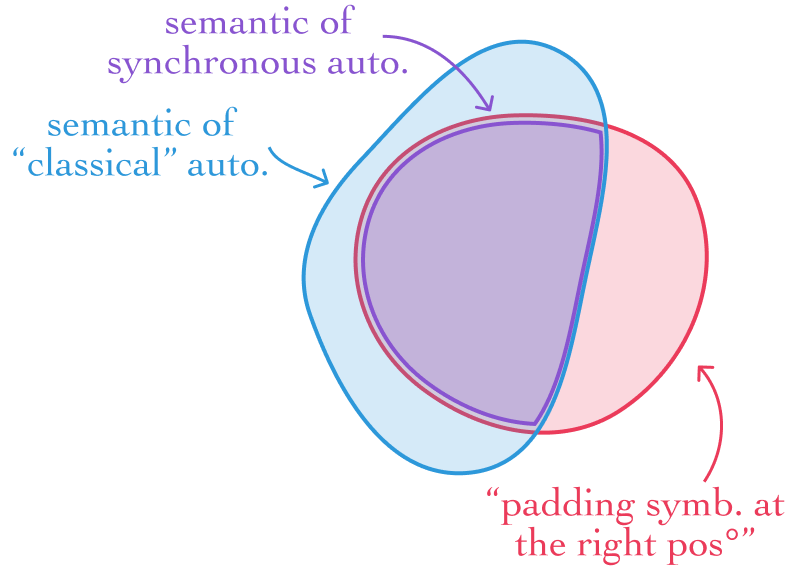
\includegraphics[width=\linewidth]{fig/intro/projection.png}
	\caption{\AP\label{fig:intro-projection}
		Semantics of a "synchronous automaton".
	}
\end{marginfigure}
This approach is ubiquitous in mathematics, and especially in logics:
for instance, first-order logic over "finite structures" is precisely
defined as first-order logic over all "structures", restricted to "finite structures"!
While being natural and ubiquitous, this construction fails to preserve most properties of the logics:
for instance, first-order logic over all "structures" admits a complete proof system,
but does not when restricted to "finite structures". The model-checking problem
is "coRE"-complete over all "structures", but goes to
"RE"-complete---an incomparable complexity class---for "finite structures".
Proving a meta-theorem on such a restriction that explains how some property
behaves in the restricted universe simply by knowing how it behaves on
the larger universe is hence somewhat unexpected but very welcomed!

\begin{contribution}
	We prove that, for any class of "regular languages" satisfying mild closure
	properties, assuming we can decide if a language belongs to this class,
	then we can decide if an "automatic relation" can be written as the restriction
	of a "regular language" in this class to the set of all valid encodings
	of pairs of words.
\end{contribution}

Let us point out that actually, to arrive at this result the notion
of "synchronous algebras" is somewhat intricate. While a more naive definition
exists and makes sense, we show that such a result cannot be proven using this
simpler notion.

This algebraic theory could provide an interesting framework to
study the "$\AUT$/$\REC$-separability problem".
While the class of "recognizable relations" has some desirable
closure properties we need, it lacks others:
unfortunately, it implies that proving the decidability of
the "$\AUT$/$\REC$-separability problem" "via" this framework would
be highly non-trivial.

\begin{openproblemintro}
	Can we decide, given two "automatic relations", if they are "separable@@rel"
	by a "recognizable relation"?
\end{openproblemintro}

In summary, this thesis explores two fundamental perspectives on "homomorphism problems":
the first extends the theory of "conjunctive queries" in database theory by adding regular path
predicates, to capture natural query languages for human-centered graph-shaped data.
It focuses on the problem of query minimization, both in terms of
its total number of atoms, or its tree-width, which is a relevant parameter to
capture the complexity of its evaluation.
The second part focuses on the complexity of problems related to constraint satisfaction
over automatic structures. We show that most \emph{structural} problems, probing the shape of the 
infinite object at hand, are undecidable. In contrast, \emph{language-theoretic} 
problems, dealing with how these infinite structures are represented---or rather how easy it
is to represent them---, remain decidable.
